\chapter{Advanced Algorithms}
\label{chap:advanced_algorithms}

\begin{figure}[ht]
	\hfill
	\begin{minipage}{0.5\textwidth}
		\centering
		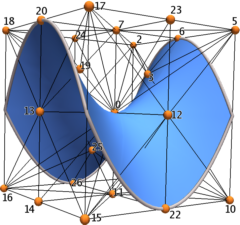
\includegraphics{VTKTextbook-168}
		\caption*{\texttt{An isocontour of a tri--quadratic Lagrange--interpolantion. Image courtesy D. Thompson and P. Pébay Sandia National Labs.}}
	\end{minipage}
\end{figure}

\firstletter{W}e return again to visualization algorithms.
This chapter describes algorithms that are either more complex to implement, or less widely used for 3D visualization applications.
We retain the classification of algorithms as either scalar, vector, tensor, or modelling algorithms.

\section{Scalar Algorithms}

As we have seen, scalar algorithms often involve mapping scalar values through a lookup table, or creating contour lines or surfaces.
In this section, we examine another contouring algorithm, dividing cubes , which generates contour surfaces using dense point clouds.
We also describe carpet plots.
Carpet plots are not true 3D visualization techniques, but are widely used to visualize many types of scalar data.
Finally, clipping is another important algorithm related to contouring, where cells are cut into pieces as a function of scalar value.

\subsection{Dividing Cubes}

Dividing cubes is a contouring algorithm similar to marching cubes \cite{Cline88}. Unlike marching cubes, dividing cubes generates point primitives as compared to triangles (3D) or lines (2D). If the number of points on the contour surface is large, the rendered appearance of the contour surface appears ``solid''.
To achieve this solid appearance, the density of the points must be at or greater than screen resolution. (Also, the points must be rendered using the standard lighting and shading equations used in surface rendering.)

The motivation for dividing cubes is that rendering points is much faster than rendering polygons. This varies depending upon rendering hardware/software. Special purpose hardware has been developed to render shaded points at high speed. In other systems, greater attention has been placed on polygon rendering, and the rendering speed differences are not so great. Also, certain geometric operations such as clipping and merging data are simple operations with points. Comparable operations with polygons are much more difficult to implement.

One disadvantage of creating contours with dense point clouds is that magnification of the surface (via camera zooming, for example) reveals the disconnected nature of the surface. Thus, the point set must be constructed for maximum zoom, or constructed dynamically based on the relative relationship between the camera and contour.

Although dividing cubes was originally developed for volume datasets, it is possible to adapt the algorithm to other dataset types by subdividing in parametric coordinates. Our presentation assumes that we are working with volumes.

\begin{figure}[!htb]
    \centering
    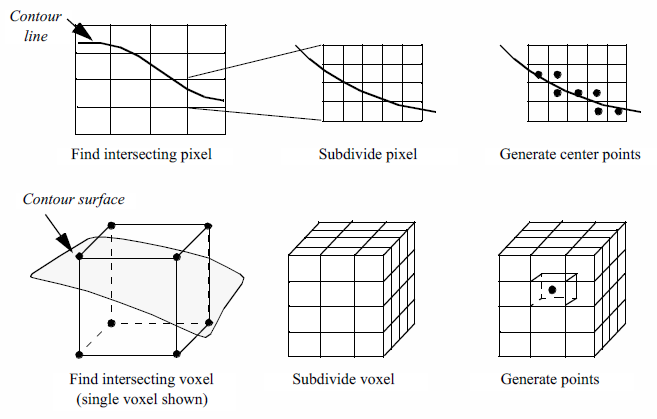
\includegraphics[width=0.98\textwidth]{Figure9-1}\\
    \caption{Overview of the dividing cubes algorithm. Voxels through which the contour passes are subdivided into subvoxels at less than screen resolution. If the contour passes through a subvoxel, a center point is generated.}\label{fig:Figure9-1}
\end{figure}

Figure \ref{fig:Figure9-1} provides an overview of the dividing cubes algorithm. Like other contouring algorithms, we first choose a contour value. We begin by visiting each voxel and select those through which the isosurface passes. (The isosurface passes through a voxel when there are scalar values both above and below the contour value.) We also compute the gradient at each voxel point for use in computing point normals.

After selecting a voxel that the isosurface passes through, the voxel is subdivided into a regular grid of $n1 \times n2 \times n3$ subvoxels. The number of divisions is controlled by the width of a voxel $w_i$ in combination with screen resolution $R$. The screen resolution is defined as the distance between adjacent pixels in world coordinates. We can express the number of divisions ni along the coordinate axes $x_i$ as $w_i$

\begin{equation}\label{eq:9.1}
n_i = \dfrac{w_i}{R}
\end{equation}
\myequations{Number of divisions along a coordinate axis.}

where the quotient is rounded up to the nearest integer. The scalar values at the subpoints are generated using the interpolation functions for a voxel (see Figure \ref{fig:Figure8-10}). Then we determine whether the contour passes through each subvoxel. If it does, we simply generate a point at the center of the subvoxel and compute its normal using the standard interpolation functions.

\begin{figure}[!htb]
    \centering
    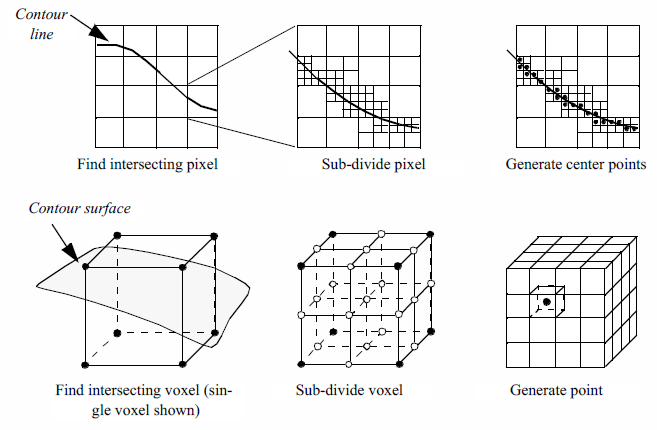
\includegraphics[width=0.98\textwidth]{Figure9-2}\\
    \caption{Recursive dividing cubes algorithm. Top half of figure shows algorithm depicted in two dimensions. Lower half depicts algorithm in three dimensions.}\label{fig:Figure9-2}
\end{figure}

An interesting variation on this algorithm is a recursive implementation as shown in Figure \ref{fig:Figure9-2}. Instead of subdividing the voxel directly (i.e., procedurally) into a regular grid we recursively divide the voxel (similar to octree decomposition). The voxel is subdivided regularly creating eight subvoxels and 19 new points (12 midedge points, 6 midface points, and 1 midvoxel point). The scalar values at the new points are interpolated from the original voxel using the trilinear interpolation functions. The process repeats for each subvoxel if the isosurface passes through it. This process continues until the size of the subvoxel is less than or equal to screen resolution. In this case, a point is generated at the center of the subvoxel. The collection of all such points composes the dividing cube's isosurface.

The advantage of the recursive implementation is that the subdivision process terminates prematurely in those regions of the voxel where the contour cannot pass. On the other hand, the recursive subdivision requires that the voxel subdivision occurs in powers of two. This can generate far more points than the procedural implementation.

\begin{figure}[!htb]
    \centering
    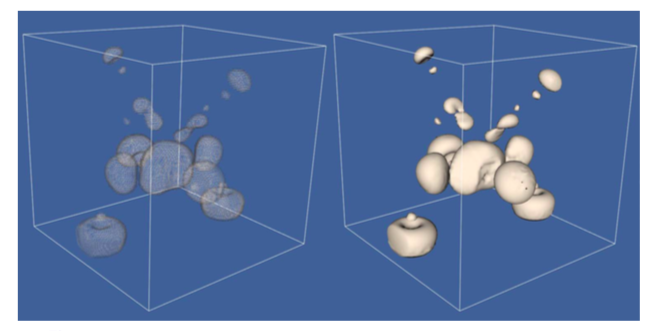
\includegraphics[width=0.98\textwidth]{Figure9-3}\\
    \caption{Examples of dividing cubes isosurface. The left image consists of 50,078 points, and the right image consists of 2,506,989 points.}\label{fig:Figure9-3}
\end{figure}

Figure \ref{fig:Figure9-3} shows two examples of dividing cubes isosurfaces. The contour surface on the left consists of 50,078 points. Because the points are not generated at display resolution, it is possible to see through the contour surface. The second contour surface on the right is composed of 2,506,989 points. The points are generated at display resolution, and as a result the contour surface appears solid.

As Figure \ref{fig:Figure9-1} and Figure \ref{fig:Figure9-2} show, the points generated by dividing cubes do not lie exactly on the contour surface. We can determine the maximum error by examining the size of the terminal subvoxels. Assume that a terminal subvoxel is a cube, and that the length of the side of the cube is given by $l$. Then the maximum error is half the length of the cube diagonal, or $l \sqrt{3} / 2$.

\subsection{Carpet Plots}

A common data form is a 2D image dataset with associated scalar data. Carpet plots can visualize data in this form. A carpet plot is created by warping a 2D surface in the direction of the surface normal (or possibly some user-defined direction). The amount of warping is controlled by the scalar value, possibly in combination with a scale factor. Carpet plots are similar to the vector displacement plots (see ``Displacement Plots'' on page \pageref{subsec:displacement_plots})

Although carpet plots are typically applied to image data, they can be used to visualize datasets composed of 2D structured grids or 2D unstructured grids. In their basic form carpet plots can be used to visualize only three variables: two surface position coordinates and a scalar value. However, it is common to introduce another variable by using color mapping on the surface.

\begin{figure}[!htb]
    \centering
    \begin{subfigure}{0.48\linewidth}
        \centering
        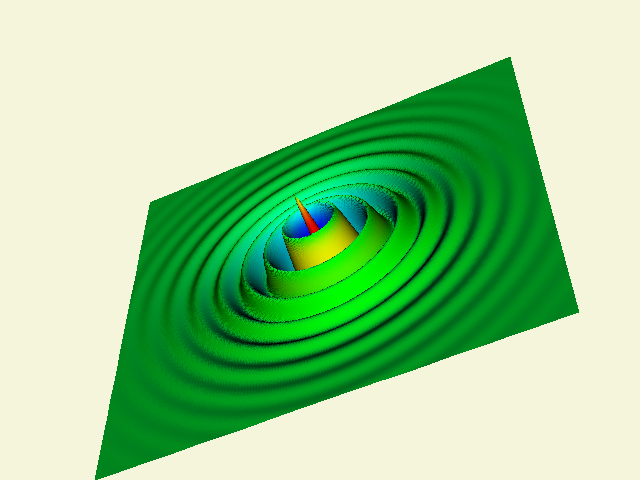
\includegraphics[width=.96\linewidth]{Figure9-4a}
        \caption{Exponential cosine function.(\href{https://lorensen.github.io/VTKExamples/site/Cxx/VisualizationAlgorithms/ExponentialCosine/}{ExponentialCosine.cxx} or \href{https://lorensen.github.io/VTKExamples/site/Python/VisualizationAlgorithms/ExponentialCosine/}{ExponentialCosine.py})}\label{fig:Figure9-4a}
    \end{subfigure}
    \hfill
    \begin{subfigure}{0.48\linewidth}
        \centering
        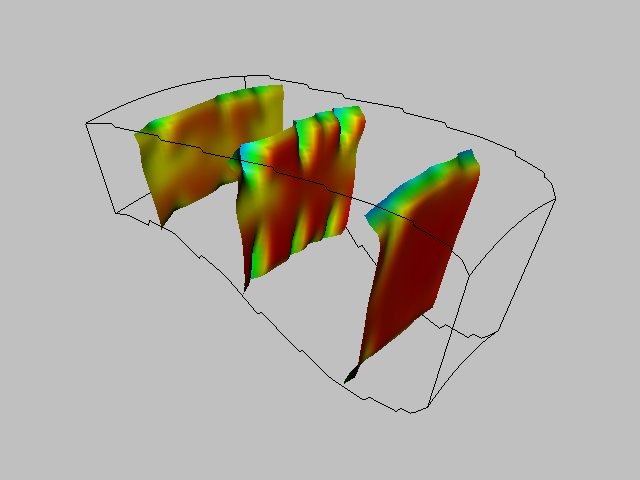
\includegraphics[width=.96\linewidth]{Figure9-4b}
        \caption{Flow energy.(\href{https://lorensen.github.io/VTKExamples/site/Cxx/VisualizationAlgorithms/WarpCombustor/}{WarpCombustor.cxx} or \href{https://lorensen.github.io/VTKExamples/site/Python/VisualizationAlgorithms/WarpCombustor/}{WarpCombustor.py})}\label{fig:Figure9-4b}
    \end{subfigure}%
    \caption{Carpet plot. (a) Visualization of an exponential cosine function. Function values are indicated by surface displacement. Colors indicate derivative values. Carpet plot of combustor flow energy in a structured grid. Colors and plane displacement represent energy values.}
    \label{fig:Figure9-4}
\end{figure}

Figure \ref{fig:Figure9-4} illustrates application of carpet plots. Figure \ref{fig:Figure9-4}(a) shows the exponential cosine function centered at the origin with points located at radius $r$

\begin{equation}\label{eq:9.2}
F(r) = e^{-r}\cos(10\, r)
\end{equation}
\myequations{Exponential cosine function.}

The function values are used to warp the surface while the function derivatives are used to color it. Figure \ref{fig:Figure9-4}(b) shows a carpet plot that visualizes flow energy in a structured grid. Both displacement and color are used to show the energy values. Although this figure is similar to Figure \ref{fig:Figure6-14}(b) there are some important differences. Figure \ref{fig:Figure6-14}(b) displays vector data whereas Figure \ref{fig:Figure9-4}(b) displays scalar data. Figure \ref{fig:Figure9-4}(b) deforms the surface in the direction of surface normal (or possibly a user-defined direction). The vector data (i.e., vector orientation) controls the direction of deformation in Figure \ref{fig:Figure6-14}(b).

\subsection{Clipping With Scalar Fields}
\label{subsec:clipping_with_scalar_fields}

\begin{figure}[!htb]
    \centering
    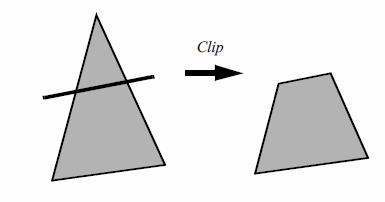
\includegraphics[width=0.98\textwidth]{Figure9-5}\\
    \caption{Clipping a triangle produces a polygon. The dark line represents an infinite plane.}\label{fig:Figure9-5}
\end{figure}


Clipping is a common graphics operation that limits the extent of a polygon so that it does not lie outside the view frustrum (see on page ``Cameras'' on page \pageref{sec:cameras}). Figure \ref{fig:Figure9-5} shows a triangle before and after clipping with an infinite plane. The clip operation transforms a polygon into a polygon. Clipping can also be a powerful modeling tool. Clipping part of a structure can reveal internal details of the surface or other parts contained within the surface. Objects can be split into pieces and the pieces can be individually moved and controlled.

\begin{figure}[!htb]
    \centering
    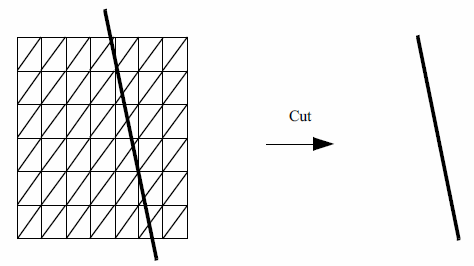
\includegraphics[width=0.98\textwidth]{Figure9-6}\\
    \caption{Cutting polygons produces lines (cutPlane.tcl).}\label{fig:Figure9-6}
\end{figure}

\begin{figure}[!htb]
    \centering
    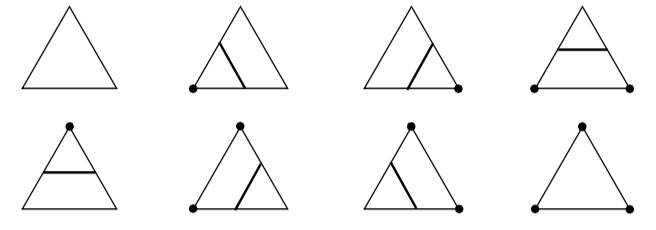
\includegraphics[width=0.98\textwidth]{Figure9-7}\\
    \caption{The eight cases for cutting (contouring) a triangle. Black dots show triangle vertices that are ``inside'' the scalar cutting region. Solid lines show the output of the cutting operation.}\label{fig:Figure9-7}
\end{figure}

We can do clipping with arbitrary implicit functions using a variation of the ``marching'' primitives discussed in ``Contouring''on page \ref{subsec:contouring}. We illustrate the technique for triangles.

Recall that marching triangles transforms triangles into lines that approximate a scalar value called the isovalue. This is accomplished using the inside/outside relationship that each vertex has with respect to some scalar value. For our purposes here, we use a scalar value that represents the signed distance of the triangle vertex to a plane. This infinite plane, described by an implicit function of the form $F(x, y, z) = n_{xx} + n_{yy} + n_{zz} - d = 0$, partitions space into two infinite half spaces. All points with negative scalar values lie on one side of the plane and all with positive values lie on the other side. Figure \ref{fig:Figure9-6} shows a finite plane represented by a grid of triangles. The thick line shows the infinite plane defined by $F(x,y,z) = x + y + z - c = 0$. The cut algorithm described in ``Cutting'' on page \pageref{subsec:cutting} creates a set of lines using the contour operations specific to each cell primitive. In this example, the triangle's contour operator extracts lines that lie on the intersection of the infinite plane and the triangles that comprise the finite plane. The contour operation for a triangle uses the eight cases shown in Figure \ref{fig:Figure9-7} to contour or ``cut'' each triangle appropriately.

\begin{figure}[!htb]
    \centering
    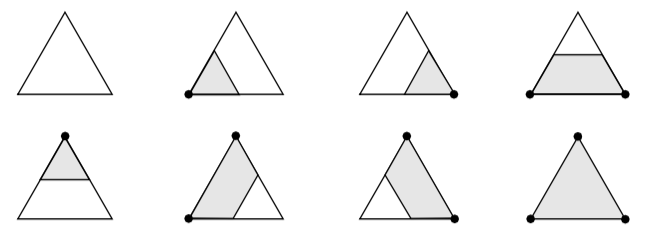
\includegraphics[width=0.98\textwidth]{Figure9-8}\\
    \caption{The eight cases for clipping a triangle. Black dots show triangle vertices that are ``inside'' the scalar clipping region. Shaded regions show the output of the clip operation.}\label{fig:Figure9-8}
\end{figure}

\begin{figure}[!htb]
    \centering
    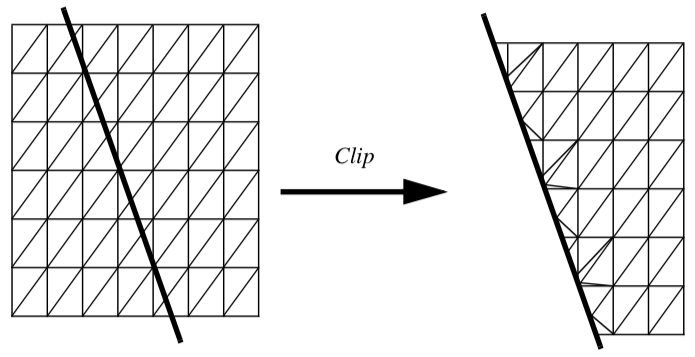
\includegraphics[width=0.98\textwidth]{Figure9-9}\\
    \caption{A plane of triangles clipped with a plane function (clipPlane.tcl).}\label{fig:Figure9-9}
\end{figure}

Clipping transforms polygons into polygons. We do clipping with a modified case table for the triangle that outputs polygons shown in Figure \ref{fig:Figure9-8}. In VTK, each polygonal data cell has a different case table to define the clip operation. Applying the clip algorithm to the polygonal data in Figure \ref{fig:Figure9-9} using the same scalar field generated with a plane equation produces a new set of triangles.

Formulating clipping using scalar fields permits more sophisticated operations. Clipping can use scalar data that is computed or scalar data that is part of a polygonal dataset's point attributes.

\begin{figure}[!htb]
    \centering
    \begin{subfigure}{0.41\linewidth}
        \centering
        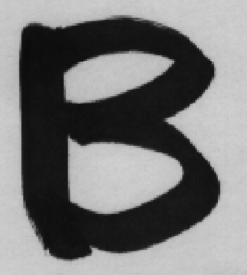
\includegraphics[width=.96\linewidth]{Figure9-10a}
        \caption*{}\label{fig:Figure9-10a}
    \end{subfigure}
    \hfill
    \begin{subfigure}{0.16\linewidth}
        \centering
        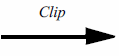
\includegraphics[width=.96\linewidth]{Figure9-10b}
        \caption*{}\label{fig:Figure9-10b}
    \end{subfigure}%
    \hfill
    \begin{subfigure}{0.41\linewidth}
        \centering
        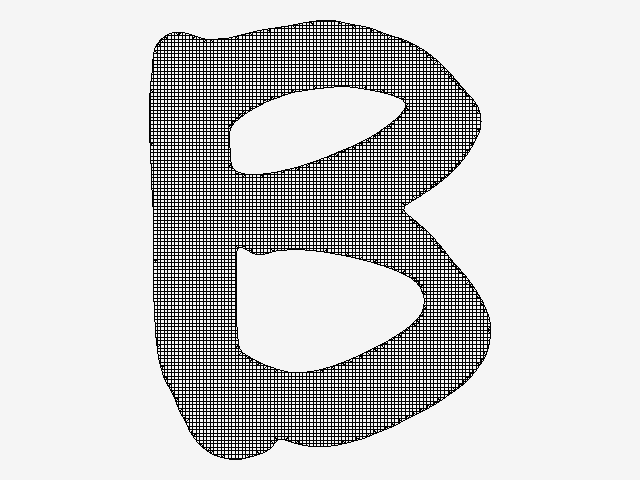
\includegraphics[width=.96\linewidth]{Figure9-10c}
        \caption*{(\href{https://lorensen.github.io/VTKExamples/site/Cxx/VisualizationAlgorithms/CreateBFont/}{CreateBFont.cxx} or \href{https://lorensen.github.io/VTKExamples/site/Python/VisualizationAlgorithms/CreateBFont/}{CreateBFont.py})}\label{fig:Figure9-10c}
    \end{subfigure}%
    \caption{Carpet plot. (a) Visualization of an exponential cosine function. Function values are indicated by surface displacement. Colors indicate derivative values. Carpet plot of combustor flow energy in a structured grid. Colors and plane displacement represent energy values.}
    \label{fig:Figure9-10}
\end{figure}

Figure \ref{fig:Figure9-10} shows a scanned image that is first converted to a quadrilateral mesh with vertex scalar values set to the scanned image intensity. Clipping this quadrilateral mesh with a value equal to 1/2 the maximum intensity of the scanned image produces a polygonal model show in Figure \ref{fig:Figure9-10}.

\section{Vector Algorithms}

In Chapter 6: \nameref{chap:fundamental_algorithms} we showed how to create simple vector glyphs and how to integrate particles through a vector field to create streamlines. In this section we extend these concepts to create streamribbons and streampolygons. In addition, we introduce the concept of vector field topology, and show how to characterize a vector field using topological constructs.

\subsection{Streamribbons and Streamsurfaces}

Streamlines depict particle paths in a vector field. By coloring these lines, or creating local glyphs (such as dashed lines or oriented cones), we can represent additional scalar and temporal information. However, these techniques can convey only elementary information about the vector field. Local information (e.g., flow rotation or derivatives) and global information (e.g., structure of a field such as vortex tubes) is not represented. Streamribbons and streamsurfaces are two techniques used to represent local and global information.

A natural extension of the streamline technique widens the line to create a ribbon. The ribbon can be constructed by generating two adjacent streamlines and then bridging the lines with a polygonal mesh. This technique works well as long as the streamlines remain relatively close to one another. If separation occurs, so that the streamlines diverge, the resulting ribbon will not accurately represent the flow, because we expect the surface of the ribbon to be everywhere tangent to the vector field (i.e., definition of streamline). The ruled surface connecting two widely separated streamlines does not generally satisfy this requirement.

The streamribbon provides information about important flow parameters: the vector vorticity and flow divergence. \emph{Vorticity} $\Omega$ is the measure of rotation of the vector field, expressed as a vector quantity: a direction (axis of rotation) and magnitude (amount of rotation). \emph{Streamwise vorticity} $\Omega$ is the projection of $\overrightarrow{\omega}$ along the instantaneous velocity vector, $\overrightarrow{v}$. Said another way, streamwise vorticity is the rotation of the vector field around the streamline defined as follows.

\begin{equation}\label{eq:9.3}
\Omega = \frac{\overrightarrow{v\ } \cdot \overrightarrow{\omega\ }}{\vert \overrightarrow{v\ } \vert \vert \overrightarrow{\omega\ } \vert}
\end{equation}
\myequations{Streamwise vorticity.}

The amount of twisting of the streamribbon approximates the streamwise vorticity. Flow divergence is a measure of the ``spread'' of the flow. The changing width of the streamribbon is proportional to the cross-flow divergence of the flow.

A streamsurface is a collection of an infinite number of streamlines passing through a \emph{base curve}. The base curve, or \emph{rake}, defines the starting points for the streamlines. If the base curve is closed (e.g., a circle) the surface is closed and a streamtube results. Thus, streamribbons are specialized types of streamsurfaces with a narrow width compared to length.

Compared to vector icons or streamlines, streamsurfaces provide additional information about the structure of the vector field. Any point on the streamsurface is tangent to the velocity vector. Consequently, taking an example from fluid flow, no fluid can pass through the surface. Streamtubes are then representations of constant mass flux. Streamsurfaces show vector field structure better than streamlines or vector glyphs because they do not require visual interpolation across icons.

Streamsurfaces can be computed by generating a set of streamlines from a user-specified rake. A polygonal mesh is then constructed by connecting adjacent streamlines. One difficulty with this approach is that local vector field divergence can cause streamlines to separate. Separation can introduce large errors into the surface, or possibly cause self-intersection, which is not physically possible.

Another approach to computing streamsurfaces has been taken by Hultquist \cite{Hultquist92}. The streamsurface is a collection of streamribbons connected along their edges. In this approach, the computation of the streamlines and tiling of the streamsurface is carried out concurrently. This allows streamlines to be added or removed as the flow separates or converges. The tiling can also be controlled to prevent the generation of long, skinny triangles. The surface may also be ``torn'', i.e., ribbons separated, if the divergence of the flow becomes too high.

\subsection{Stream Polygon}

he techniques described so far provide approximate measures of vector field quantities such as streamwise vorticity and divergence. However, vector fields contain more information than these techniques can convey. As a result, other techniques have been devised to visualize this information. One such technique is the stream polygon \cite{Schroeder91}, which serves as the basis for a number of advanced vector and tensor visualization methods. The stream polygon is used to visualize local properties of strain, displacement, and rotation. We begin by describing the effects of a vector field on the local state of strain.

Nonuniform vector fields give rise to local deformation in the region where they occur. If the vector field is displacement in a physical medium such as a fluid or a solid, the deformation consists of local strain (i.e., local distortion) and rigid body motion. To mathematically describe the deformation, we examine a 3D vector $\overrightarrow{v\ } = (u, v, w)$ at a specified point $x = (x, y, z)$. Using a first order Taylor's series expansion about $\overrightarrow{x\ }$, we can express the local deformation $e_ij$ as

\begin{equation}\label{eq:9.4}
e_{ij} = \epsilon_{ij} + \omega_{ij}
\end{equation}
\myequations{Local deformation.}

where $\epsilon_{ij}$ is the local strain and $\omega_{ij}$ is the local rotation. Note that these variables are expressed as $3 \times 3$ tensors. (Compare this equation to that given in Figure \ref{fig:Figure6-20}. Note that this equation and the following Equation \ref{eq:9.5} differ in their off-diagonal terms by a factor of $1/2$. This is because Figure \ref{fig:Figure6-20} expresses engineering shear strain which is used in the study of elasticity. Equation \ref{eq:9.5} expresses a tensor quantity and is mathematically consistent.)

The local strain is expressed as a combination of the partial derivatives at $\overrightarrow{x\ }$ as follows.

\begin{equation}\label{eq:9.5}
\mathbf{\epsilon} = \left(
\begin{array}{c c c}
  \dfrac{\partial u}{\partial x} &
  \dfrac{1}{2}\left(\dfrac{\partial u}{\partial y} + \dfrac{\partial v}{\partial x}\right) &
  \dfrac{1}{2}\left(\dfrac{\partial u}{\partial z} + \dfrac{\partial w}{\partial x}\right) \\ \\
  \dfrac{1}{2}\left(\dfrac{\partial u}{\partial y} + \dfrac{\partial v}{\partial x}\right) &
  \dfrac{\partial v}{\partial y} &
  \dfrac{1}{2}\left(\dfrac{\partial v}{\partial z} + \dfrac{\partial w}{\partial y}\right) \\ \\
  \dfrac{1}{2}\left(\dfrac{\partial u}{\partial z} + \dfrac{\partial w}{\partial x}\right) &
  \dfrac{1}{2}\left(\dfrac{\partial v}{\partial z} + \dfrac{\partial w}{\partial y}\right) &
  \dfrac{\partial w}{\partial z}
\end{array}\right)
\end{equation}
\myequations{Local strain.}

The terms on the diagonal of $\epsilon_{ij}$ are the normal components of strain. The off-diagonal terms are the shear strain. The local rigid--body rotation is given by

\begin{equation}\label{eq:9.6}
\mathbf{\omega} = \left(
\begin{array}{c c c}
  0 &
  \dfrac{1}{2}\left(\dfrac{\partial u}{\partial y} - \dfrac{\partial v}{\partial x}\right) &
  \dfrac{1}{2}\left(\dfrac{\partial u}{\partial z} - \dfrac{\partial w}{\partial x}\right) \\ \\
  \dfrac{1}{2}\left(\dfrac{\partial v}{\partial x} - \dfrac{\partial u}{\partial y}\right) &
  0 &
  \dfrac{1}{2}\left(\dfrac{\partial v}{\partial z} - \dfrac{\partial w}{\partial y}\right) \\ \\
  \dfrac{1}{2}\left(\dfrac{\partial w}{\partial x} - \dfrac{\partial u}{\partial z}\right) &
  \dfrac{1}{2}\left(\dfrac{\partial w}{\partial y} - \dfrac{\partial v}{\partial z}\right) &
  0
\end{array}\right)
\end{equation}
\myequations{Local rigid--body rotation.}

Equation \ref{eq:9.6} can also be represented using tensor notation as

\begin{equation}\label{eq:9.7}
\omega_{ij} = -\dfrac{1}{2}\sum_{k} \epsilon_{ijk}\, \omega_{k}
\end{equation}
\myequations{Local deformation.}

where $\overrightarrow{\omega\ }$ is the vorticity vector referred to in the previous section. The vorticity, or local rigid body rotation is then

\begin{equation}\label{eq:9.8}
\overrightarrow{\omega\ } = \left(
\begin{array}{c}
\dfrac{\partial w}{\partial y} - \dfrac{\partial v}{\partial z} \\ \\
\dfrac{\partial u}{\partial z} - \dfrac{\partial w}{\partial x} \\ \\
\dfrac{\partial v}{\partial x} - \dfrac{\partial u}{\partial y}
\end{array}
\right)
\end{equation}
\myequations{Vorticity vector.}

\begin{figure}[htb]
	\begin{subfigure}[h]{0.48\linewidth}
		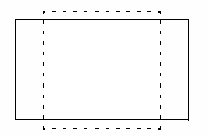
\includegraphics[width=0.96\linewidth]{Figure9-11a}
		\captionsetup{justification=centering}
		\caption{Normal strain}
		\label{fig:Figure9-11a}
	\end{subfigure}
	\hfill
	\begin{subfigure}[h]{0.48\linewidth}
		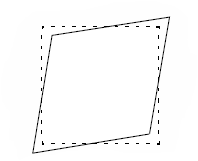
\includegraphics[width=0.96\linewidth]{Figure9-11b}
		\captionsetup{justification=centering}
		\caption{Shear strain}
		\label{fig:Figure9-11b}
	\end{subfigure}
	\hfill
	\begin{subfigure}[h]{0.48\linewidth}
		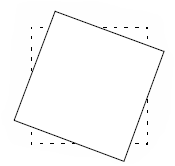
\includegraphics[width=0.96\linewidth]{Figure9-11c}
		\captionsetup{justification=centering}
		\caption{Rotation}
		\label{fig:Figure9-11c}
	\end{subfigure}
	\hfill
		\begin{subfigure}[h]{0.48\linewidth}
		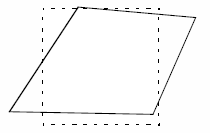
\includegraphics[width=0.96\linewidth]{Figure9-11d}
		\captionsetup{justification=centering}
		\caption{Total deformation}
		\label{fig:Figure9-11d}
	\end{subfigure}
	\caption{Components of local deformation due to vector field. Dotted line shows initially undeformed object.}\label{fig:Figure9-11}
\end{figure}

For the reader unfamiliar with tensor notation, this presentation is certainly less than complete. However, the matrices in Equation \ref{eq:9.5} and Equation \ref{eq:9.6} directly translate into visual form, which will help clarify the concepts presented here. Referring to Figure \ref{fig:Figure9-11}, the normal strain, shear strain, and rigid body motion create distinct deformation modes. These modes combine to produce the total deformation. Modes of normal strain cause compression or extension in the direction perpendicular to a surface, while shear strains cause angular distortions. These strains combined with rigid body rotation around an axis yield the total strain at a point.

\begin{figure}[htb]
	\begin{subfigure}[h]{0.48\linewidth}
		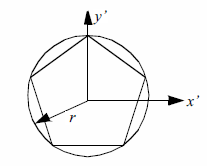
\includegraphics[width=0.96\linewidth]{Figure9-12a}
		\captionsetup{justification=centering}
		\caption{Planar view}
		\label{fig:Figure9-12a}
	\end{subfigure}
	\hfill
	\begin{subfigure}[h]{0.48\linewidth}
		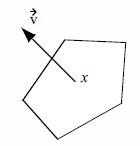
\includegraphics[width=0.96\linewidth]{Figure9-12b}
		\captionsetup{justification=centering}
		\caption{Normal to vector}
		\label{fig:Figure9-12b}
	\end{subfigure}
	\hfill
	\begin{subfigure}[h]{0.48\linewidth}
		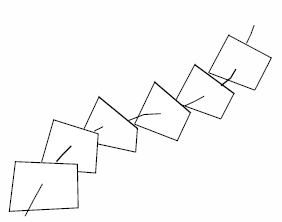
\includegraphics[width=0.96\linewidth]{Figure9-12c}
		\captionsetup{justification=centering}
		\caption{Placed along streamline}
		\label{fig:Figure9-12c}
	\end{subfigure}
	\hfill
		\begin{subfigure}[h]{0.48\linewidth}
		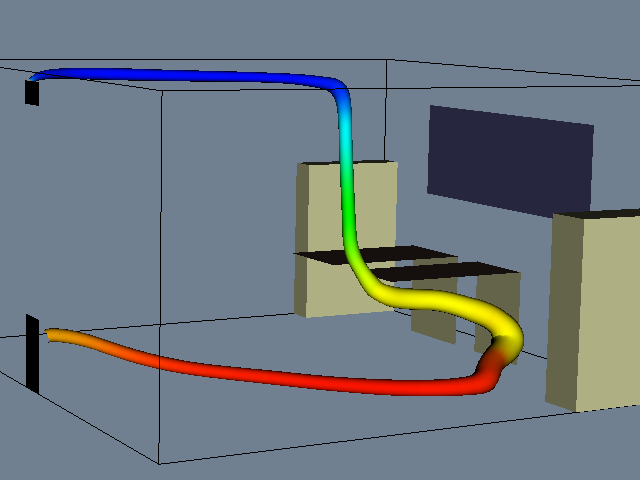
\includegraphics[width=0.96\linewidth]{Figure9-12d}
		\captionsetup{justification=centering}
		\caption{Stream tube(\href{https://lorensen.github.io/VTKExamples/site/Cxx/VisualizationAlgorithms/OfficeTube/}{OfficeTube.cxx} or \href{https://lorensen.github.io/VTKExamples/site/Python/VisualizationAlgorithms/OfficeTube/}{OfficeTube.py})}
		\label{fig:Figure9-12d}
	\end{subfigure}
	\caption{The stream polygon. (a) Planar view. (b) Aligned with vector. (c) Aligned along streamline. (d) Sweeping polygon to form tube.}\label{fig:Figure9-12}
\end{figure}

The essence of the stream polygon technique is to show these modes of deformation. A regular \emph{n}--sided polygon (Figure \ref{fig:Figure9-12}) is placed into a vector field at a specified point and then deformed according to the local strain. The components of strain may be shown separately or in combination. The orientation of the normal of the polygon is arbitrary. However, it is convenient to align the normal with the local vector. Then the rigid body rotation about the vector is the streamwise vorticity, and the effects of normal and shear strain are in the plane perpendicular to a streamline passing through the point.

The stream polygon offers other interesting possibilities. The stream polygon may be swept along a trajectory, typically a streamline, to generate tubes. The radius of the tube $r$ can be modified according to some scalar function. One application is to visualize fluid flow. In incompressible flow with no shear, the radius of the tube can vary according to the scalar function vector magnitude. Then the equation

\begin{equation}\label{eq:9.9}
r(\overrightarrow{v\ }) = r_\text{max} \sqrt{\dfrac{\vert\overrightarrow{v}_\text{min}\vert}{\vert\overrightarrow{v\ }\vert}}
\end{equation}
\myequations{Area of constant mass flow.}

represents an area of constant mass flow. As a result, the tube will thicken as the flow slows and narrow as the velocity increases. Each of the \emph{n} sides of the tube can be colored with a different scalar function, although for visual clarity, at most, one or two functions should be used.

The streamtubes generated by the streampolygon and the streamtubes we described in the previous section are not the same. The streampolygon does not necessarily lie along a streamline. If it does, the streampolygon represents information at a point, while the streamtube is an approximation constructed from multiple streamlines. Also, the radial variation in the tubes constructed from streampolygon sweeps do not necessarily relate to mass flow since the radius in a streampolygon can be tied to an arbitrary scalar variable.

\subsection{Vector Field Topology}

Vector fields have a complex structure characterized by special features called critical points \cite{Globus91} \cite{Helman91}. Critical points are locations in the vector field where the local vector magnitude goes to zero and the vector direction becomes undefined. At these points the vector field either converges or diverges, and/or local circulation around the point occurs.

Critical points lie in dataset cells where the u, v, and w components of the vector field each pass through zero. These points are located using an iterative search procedure such as the bi-section technique. Each iteration evaluates the cell interpolation function until the zero vector is found. Once a critical point is found, its local behavior is determined from the matrix of partial derivatives.

This is because at the critical point the velocity is zero, and the vector field can be approximated by a first-order expansion of partial derivatives \cite{Helman91}

\begin{equation}\label{eq:9.10}
\begin{array}{lll}
u &\simeq& \dfrac{\partial u}{\partial x}\text{d}x
         + \dfrac{\partial u}{\partial y}\text{d}y
         + \dfrac{\partial u}{\partial z}\text{d}z \\ \\
v &\simeq& \dfrac{\partial v}{\partial x}\text{d}x
         + \dfrac{\partial v}{\partial y}\text{d}y
         + \dfrac{\partial v}{\partial z}\text{d}z \\ \\
w &\simeq& \dfrac{\partial w}{\partial x}\text{d}x
         + \dfrac{\partial w}{\partial y}\text{d}y
         + \dfrac{\partial w}{\partial z}\text{d}z
\end{array}
\end{equation}
\myequations{Approximation of a vector field.}

The matrix of partial derivatives $J$ can be written in vector notation as $\partial u \partial v \partial w$

\begin{equation}\label{eq:9.11}
\overrightarrow{u\ } = \mathbf{J}\cdot\text{d}\overrightarrow{x },\quad \text{where} \quad \mathbf{J} = \left(
\begin{array}{c c c}
\dfrac{\partial u}{\partial x} & \dfrac{\partial u}{\partial y} & \dfrac{\partial u}{\partial z} \\ \\
\dfrac{\partial v}{\partial x} & \dfrac{\partial v}{\partial y} & \dfrac{\partial v}{\partial z} \\ \\
\dfrac{\partial w}{\partial x} & \dfrac{\partial w}{\partial y} & \dfrac{\partial w}{\partial z}
\end{array}
\right)
\end{equation}
\myequations{The Jacobian.}

and is referred to as the Jacobian. The behavior of the vector field in the vicinity of a critical point is characterized by the eigenvalues of $J$. The eigenvalues consist of an imaginary and real component. The imaginary component describes the rotation of the vector field around the critical point, while the real part describes the relative attraction or repulsion of the vector field to the critical point. In two dimensions the critical points are as shown in Figure\ref{fig:Figure9-13}.

\begin{figure}[htb]
	\begin{subfigure}[h]{0.32\linewidth}
		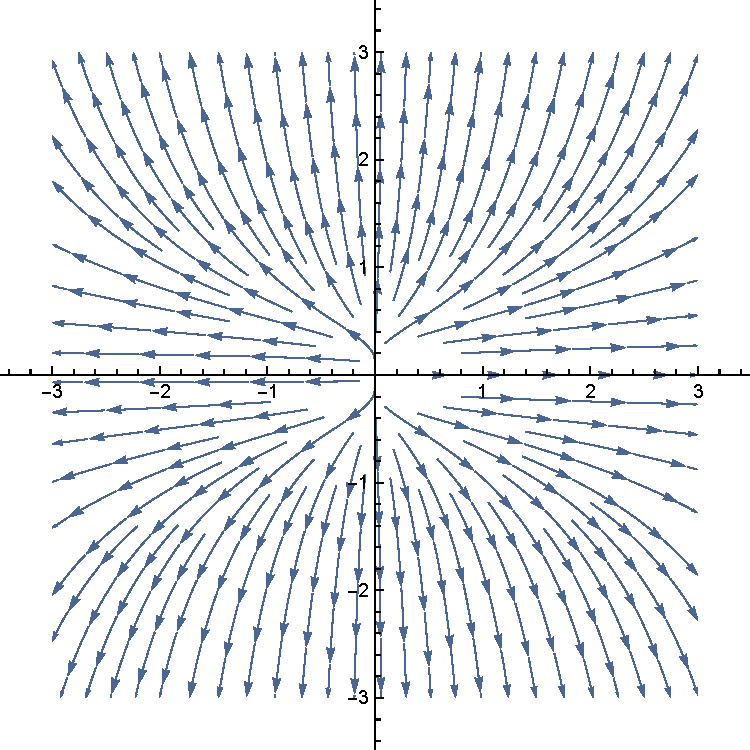
\includegraphics[width=0.86\linewidth]{Figure9-13a}
		\captionsetup{justification=centering}
		\caption*{Repelling Node\\$R_1, R_2 > 0$\\$I_1, I_2 = 0$}
		\label{fig:Figure9-13a}
	\end{subfigure}
	\hfill
	\begin{subfigure}[h]{0.32\linewidth}
		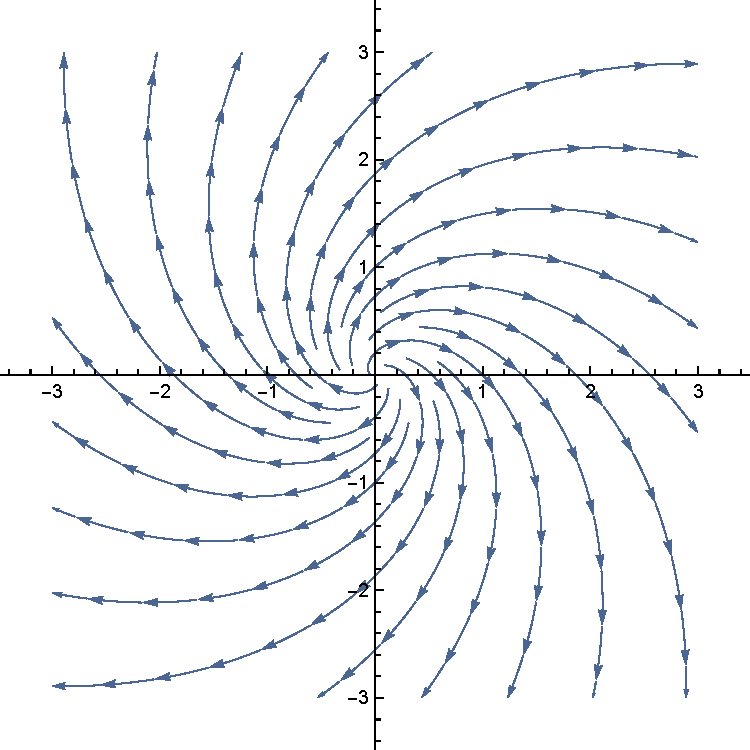
\includegraphics[width=0.86\linewidth]{Figure9-13b}
		\captionsetup{justification=centering}
		\caption*{Repelling Focus\\$R_1, R_2 > 0$\\$I_1, I_2 \neq 0$}
		\label{fig:Figure9-13b}
	\end{subfigure}
	\hfill
	\begin{subfigure}[h]{0.32\linewidth}
		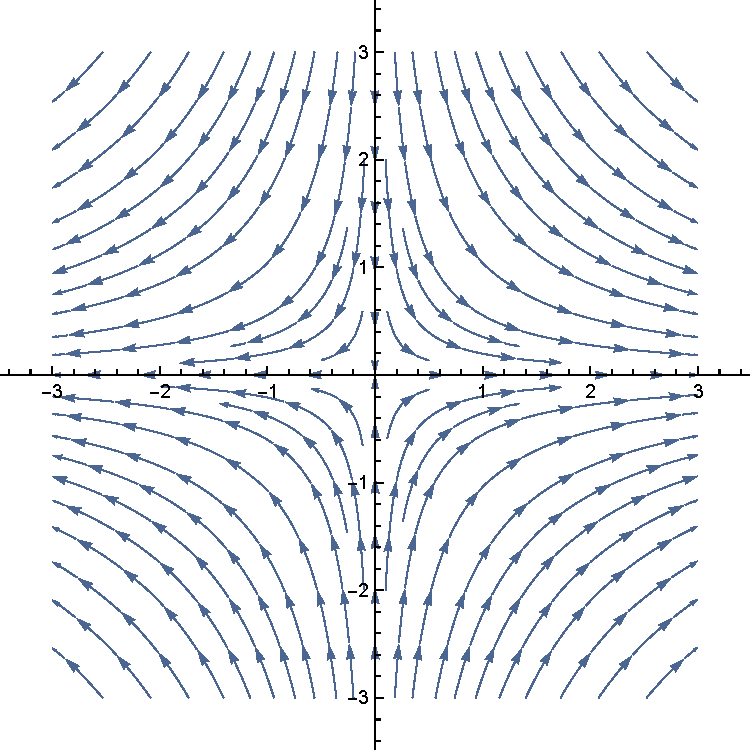
\includegraphics[width=0.86\linewidth]{Figure9-13c}
		\captionsetup{justification=centering}
		\caption*{Saddle Point\\$R_1 \times R_2 < 0$\\$I_1, I_2 = 0$}
		\label{fig:Figure9-13c}
	\end{subfigure}
	\hfill
		\begin{subfigure}[h]{0.32\linewidth}
		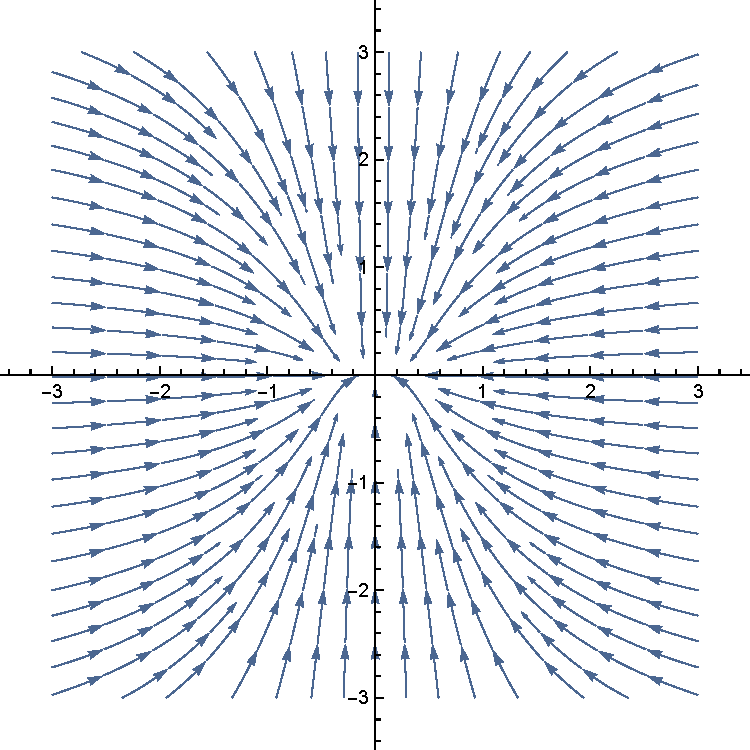
\includegraphics[width=0.86\linewidth]{Figure9-13d}
		\captionsetup{justification=centering}
		\caption*{Attracting Node\\$R_1, R_2 < 0$\\$I_1, I_2 = 0$}
		\label{fig:Figure9-13d}
	\end{subfigure}
	\hfill
	\begin{subfigure}[h]{0.32\linewidth}
		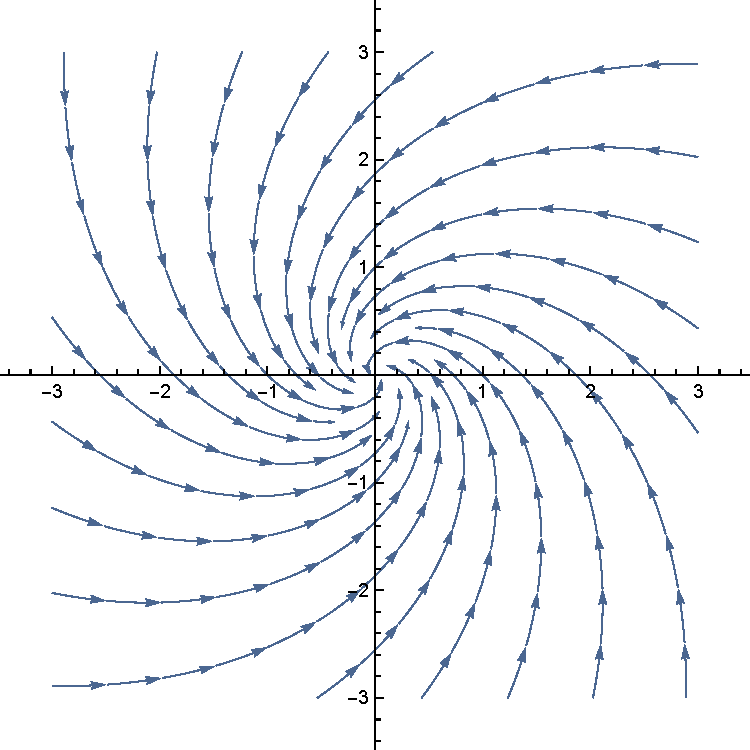
\includegraphics[width=0.86\linewidth]{Figure9-13e}
		\captionsetup{justification=centering}
		\caption*{Attracting Focus\\$R_1, R_2 < 0$\\$I_1, I_2 \neq 0$}
		\label{fig:Figure9-13e}
	\end{subfigure}
	\hfill
	\begin{subfigure}[h]{0.32\linewidth}
		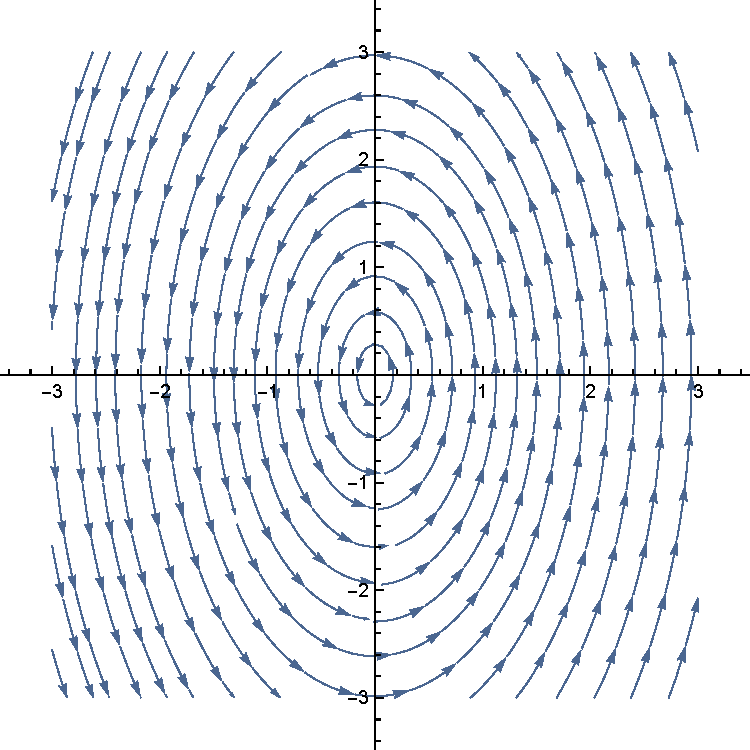
\includegraphics[width=0.86\linewidth]{Figure9-13f}
		\captionsetup{justification=centering}
		\caption*{Center\\$R_1, R_2 = 0$\\$I_1, I_2 \neq 0$}
		\label{fig:Figure9-13f}
	\end{subfigure}
	\caption{Critical points in two dimensions. The real part of the eigenvalues ($R_1$, $R_2$) of the matrix of first derivatives control the attraction or repulsion of the vector field. The imaginary part of the eigenvalues ($I_1$, $I_2$) controls the rotation.}\label{fig:Figure9-13}
\end{figure}

A number of visualization techniques have been developed to construct vector field topology from an analysis of critical points. These techniques provide a global understanding of the field, including points of attachment and detachment and field vortices. Using a fluid flow analogy, points of attachment and detachment occur on the surface of an object where the tangential component of the vector field goes to zero, and the flow is perpendicular to the surface. Thus, streamlines will begin or end at these points. There is no common definition for a vortex, but generally speaking, vortices are regions of relatively concentrated vorticity (e.g., flow rotation). The study of vortices is important because they represent areas of energy loss, or can have significant impact on downstream flow conditions (e.g., trailing vortices behind large aircraft).

One useful visualization technique creates vector field skeletons that divide the vector field into separate regions. Within each region, the vector field is topologically equivalent to uniform flow. These skeletons are created by locating critical points, and then connecting the critical points with streamlines. In 3D vector field analysis this technique can be applied to the surface of objects to locate lines of flow separation and attachment and other important flow features. Also, in general 3D flow, the regions of uniform flow are separated by surfaces, and creation of 3D flow skeletons is a current research topic.

Vortex visualization is another area of current research. One technique computes the \emph{helicitydensity}

\begin{equation}\label{eq:9.12}
H_d = \overrightarrow{v\ } \cdot \overrightarrow{w\ } = \vert \overrightarrow{v\ } \vert \vert \overrightarrow{w\ } \vert \cos(\phi)
\end{equation}
\myequations{Scalar function of the vector dot product. }

This is a scalar function of the vector dot product between the vorticity and the local vector. Large positive values of $H_d$ result in right-handed vortices, while large negative values indicate lefthanded vortices. Helicity-density can be conveniently shown using isosurfaces, which gives an indication for the location and structure of a vortex.

\section{Tensor Algorithms}

In Chapter 6: \nameref{chap:fundamental_algorithms} we saw that $3 \times 3$ real symmetric tensors can be characterized by the eigenvalues and eigenvectors of the tensor. Recall that we can express the eigenvectors of the system as

\begin{equation}\label{eq:9.13}
\overrightarrow{v\ } = \sum_i \lambda_i \overrightarrow{e\ }_i
\end{equation}
\myequations{Eigenvalues of a system. }

where $\overrightarrow{e\ }_i$ is a unit vector in the direction of the eigenvalue, and $\lambda_i$ are the eigenvalues. Thus, we can decompose a  $3 \times 3$ real symmetric tensor field into three vector fields, each field defined by one of the three eigenvectors described in Equation \ref{eq:9.13}. We call these vector fields \emph{eigenfields}, since they are derived from the eigenvectors of the tensor field.

Decomposition of the tensor field in this fashion provides additional insight into visualizing $3 \times 3$ real symmetric tensors. We can directly use the vector field visualization techniques presented previously or use variations of them. One such technique is a novel extension of the streampolygon technique, the method of \emph{hyperstreamlines}.

\subsection{Hyperstreamlines}

\begin{figure}[htb]
	\begin{subfigure}[h]{0.48\linewidth}
		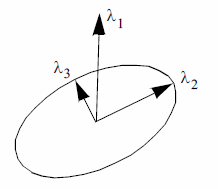
\includegraphics[width=0.66\linewidth]{Figure9-14a}
		\captionsetup{justification=centering}
		\caption{Ellipse definition}
		\label{fig:Figure9-14a}
	\end{subfigure}
	\hfill
	\begin{subfigure}[h]{0.48\linewidth}
		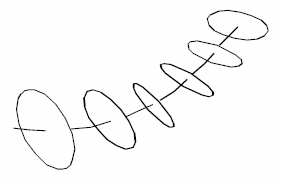
\includegraphics[width=0.96\linewidth]{Figure9-14b}
		\captionsetup{justification=centering}
		\caption{Ellipse swept to create tube}
		\label{fig:Figure9-14b}
	\end{subfigure}
	\caption{Creation of hyperstreamlines. An ellipse is swept along a streamline of the eigenfield. Major/minor axes of the ellipse are controlled by the other two eigenvectors.}\label{fig:Figure9-14}
\end{figure}

Hyperstreamlines are constructed by creating a streamline through one of the three eigenfields, and then sweeping a geometric primitive along the streamline \cite{Delmarcelle93}. Typically, an ellipse is used as the geometric primitive, where the remaining two eigenvectors define the major and minor axes of the ellipse (Figure \ref{fig:Figure9-14}). Sweeping the ellipse along the eigenfield streamline results in a tubular shape. Another useful generating geometric primitive is a cross. The length and orientation of the arms of the cross are controlled by two of the eigenvectors. Sweeping the cross results in a helical shape since the eigenvectors (and therefore cross arms) will rotate in some tensor fields.

\begin{figure}[!htb]
	\floatbox[{\capbeside\thisfloatsetup{capbesideposition={right,center},capbesidewidth=0.4\textwidth}}]{figure}[\FBwidth]
	{\caption{The four hyperstreamlines shown are integrated along the minor principle stress axis. A plane (colored with a different lookup table) is also shown.(\href{https://lorensen.github.io/VTKExamples/site/Cxx/VisualizationAlgorithms/HyperStreamline/}{HyperStreamline.cxx} or \href{https://lorensen.github.io/VTKExamples/site/Python/VisualizationAlgorithms/HyperStreamline/}{HyperStreamline.py}}\label{fig:Figure9-15}}
	{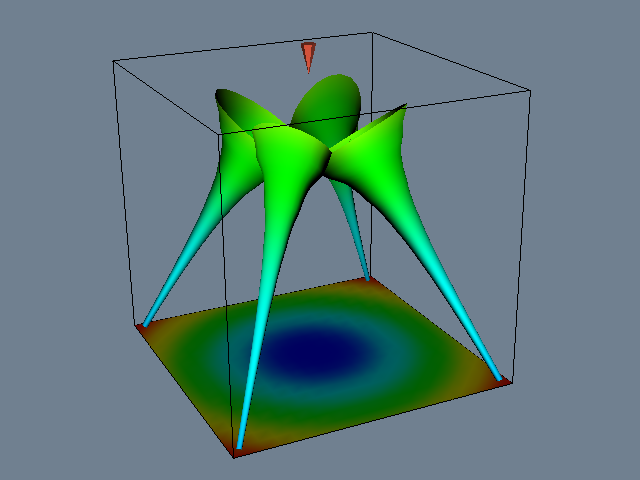
\includegraphics[width=0.6\textwidth]{Figure9-15}}
\end{figure}


Figure \ref{fig:Figure9-15} shows an example of hyperstreamlines. The data is from a point load applied to a semi-infinite domain. Compare this figure to Figure \ref{fig:Figure6-22} that used tensor ellipsoids to visualize the same data. Notice that there is less clutter and more information available from the hyperstreamline visualization.



\section{Modelling Algorithms}

\subsection{Visualizing Geometry}

One of the most common applications of visualization is to view geometry. We may have a geometric representation of a part or complex assembly (perhaps designed on a CAD system) and want to view the part or assembly before it is manufactured. While viewing geometry is better addressed in text on computer graphics, often there is dataset structure we wish to view in the same way. For example, we may want to see data mapped on a particular portion of the dataset, or view the structure of the dataset itself (e.g., view a finite element mesh).

Three-dimensional datasets have a surface and interior. Typically we want to visualize the surface of the dataset or perhaps a portion of the interior. (Note: volume rendering is a different matter - see ``Volume Rendering'' on page \pageref{sec:volume_rendering}). To visualize the dataset we must extract a portion of the dataset topology/geometry (and associated data) as some form of surface primitives such as polygons. If the surface of the dataset is opaque, we may also wish to eliminate occluded interior detail.

We have already seen how structured datasets, such as image data or structured grids, have a natural $i-j-k$ coordinate system that allow extraction of points, lines, and planes from the interior of the dataset (see ``Structured Coordinate System'' on page \pageref{subsec:structured_coordinate_system})). For example, to extract the fifth $-$iplane from a structured grid of dimensions $(i_m, j_m, k_m)$, we specify the data extents using $(4, 4, 0, (j_m - 1), 0, (k_m 1))$ (assuming zero-offset addressing).

\begin{figure}[htb]
	\begin{subfigure}[h]{0.48\linewidth}
		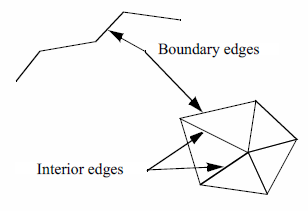
\includegraphics[width=0.96\linewidth]{Figure9-16a}
		\captionsetup{justification=centering}
		\caption*{}
		\label{fig:Figure9-16a}
	\end{subfigure}
	\hfill
	\begin{subfigure}[h]{0.48\linewidth}
		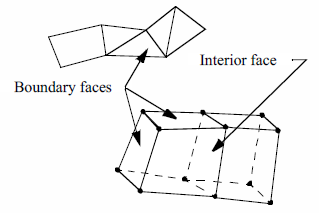
\includegraphics[width=0.96\linewidth]{Figure9-16b}
		\captionsetup{justification=centering}
		\caption*{}
		\label{fig:Figure9-16b}
	\end{subfigure}
	\caption{Boundary edges and faces.}\label{fig:Figure9-16}
\end{figure}

More generally, we can extract boundary edges and faces from a dataset. A boundary edge is an 1D cell type (e.g., line or polyline), or the edge of a 2D cell used by only that single cell. Similarly, a boundary face is a 2D cell type (e.g., polygon, triangle strip) or the face of a 3D cell used by only that single cell (Figure \ref{fig:Figure9-16}). We can obtain this information using the topological operators of the previous chapter. Cells of dimensions two or less are extracted as is, while boundary edges and faces are determined by counting the number of cell neighbors for a particular topological boundary (i.e., edge or face neighbors). If there are no neighbors, the edge or face is a boundary edge or face, and is extracted.

Using these techniques we can view the structure of our dataset. However, there are also situations where we want more control in the selection of the data. We call this \emph{data extraction}.

\subsection{Data Extraction}

Often we want to extract portions of data from a dataset. This may be because we want to reduce the size of the data, or because we are interested in visualizing only a portion of it.

Reducing dataset size is an important practical capability, because visualization data size can be huge. By reducing data size, reductions in computation and memory requirements can be realized. This results in better interactive response.

We also may need to reduce data size in order to visualize the important features of a large dataset. This can be used to reduce image clutter and improve the effectiveness of the visualization. Smaller data size also enables the visualization user to navigate through and inspect data more quickly relative to larger datasets. Next we describe two techniques to extract data. One is based on geometry extraction, and the other is based on data thresholding, or thresholding.

\subsubsection{Geometry Extraction}

Geometry extraction selects data based on geometric or topological characteristics. A common extraction technique selects a set of points and cells that lie within a specified range of ids. A typical example is selecting all cells having ids between 0-100, or all cells using point ids 250-500. Finite element analysts use this method frequently to isolate the visualization to just a few key regions.

\begin{figure}[htb]
	\begin{subfigure}[h]{0.48\linewidth}
		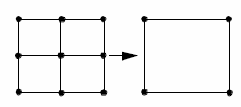
\includegraphics[width=0.96\linewidth]{Figure9-17a}
		\captionsetup{justification=centering}
		\caption{Subsampling structured data}
		\label{fig:Figure9-17a}
	\end{subfigure}
	\hfill
	\begin{subfigure}[h]{0.48\linewidth}
		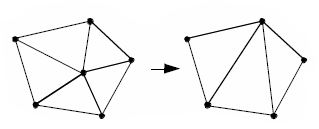
\includegraphics[width=0.96\linewidth]{Figure9-17b}
		\captionsetup{justification=centering}
		\caption{Subsampling unstructured data}
		\label{fig:Figure9-17b}
	\end{subfigure}
	\caption{Subsampling data. (a) Structured data can be subsampled by choosing every nth point. (b) Subsampling unstructured data requires local retriangulation.}\label{fig:Figure9-17}
\end{figure}

Another useful technique called spatial extraction, selects dataset structure and associated data attributes lying within a specified region in space. For example, a point and radius can be used to select (or deselect) data within an enclosing sphere. Implicit functions are particularly useful tools for describing these regions. Points that evaluate negative are inside the region, while points outside the region evaluate positive; thus, cells whose points are all positive are outside the region, and cells whose points are all negative are inside the region.

\emph{Subsampling} (Figure \ref{fig:Figure9-17}) is a method that reduces data size by selecting a subset of the original data. The subset is specified by choosing a parameter n, specifying that every nth data point is to be extracted. For example, in structured datasets such as image data and structured grids, selecting every nth point produces the results shown in igure \ref{fig:Figure9-17}(a).

Subsampling modifies the topology of a dataset. When points or cells are not selected, this leaves a topological ``hole''. Dataset topology must be modified to fill the hole. In structured data, this is simply a uniform selection across the structured $i-j-k$ coordinates. In unstructured data (Figure \ref{fig:Figure9-17}(b)), the hole must be filled in by using triangulation or other complex tessellation schemes. Subsampling is not typically performed on unstructured data because of its inherent complexity.

A related technique is \emph{data masking}. In data masking we select every $n^{th}$ cell that at a minimum leaves one or more topological ``holes'' in the dataset. Masking also may change the topology of the dataset, since partial selections of cells from structured datasets can only be represented using unstructured grids. Masking is typically used to improve interactive performance or to quickly process portions of data.

\subsubsection{Thresholding}
\label{subsubsec:thresholding}

Thresholding extracts portions of a dataset data based on attribute values. For example, we may select all cells having a point with scalar value between (0,1) or all points having a velocity magnitude greater than 1.0.

Scalar thresholding is easily implemented. The threshold is either a single value that scalar values are greater than or less than, or a range of values. Cells or points whose associated scalar values satisfy the threshold criteria can be extracted. Other dataset attribute types such as vectors, normals, or tensors can be extracted in similar fashion by converting the type to a single scalar value. For example, vectors can be extracted using vector magnitude, and tensors using matrix determinate.

A problem with both geometry extraction and thresholding is that the approaches presented thus far extract ``atomic'' pieces of data, that is, a complete cell. Sometimes the cell may lie across the boundary of the threshold. In this case the cell must be clipped (see ``Clipping With Scalar Fields'' on page \pageref{subsec:clipping_with_scalar_fields} and only a portion of the cell is extracted.

\subsection{Probing}
\label{subsec:probing}

Probing obtains dataset attributes by sampling one dataset (the input) with a set of points (the probe) as shown in Figure \ref{fig:Figure9-18}(a). Probing is also called ``resampling''. Examples include probing an input dataset with a sequence of points along a line, on a plane, or in a volume. The result of the probing is a new dataset (the output) with the topological and geometric structure of the probe dataset, and point attributes interpolated from the input dataset. Once the probing operation is completed, the output dataset can be visualized with any of the appropriate techniques described in this text.

\begin{figure}[htb]
	\begin{subfigure}[h]{0.48\linewidth}
		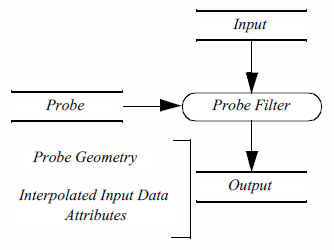
\includegraphics[width=0.96\linewidth]{Figure9-18a}
		\captionsetup{justification=centering}
		\caption{Probing process}
		\label{fig:Figure9-18a}
	\end{subfigure}
	\hfill
	\begin{subfigure}[h]{0.48\linewidth}
		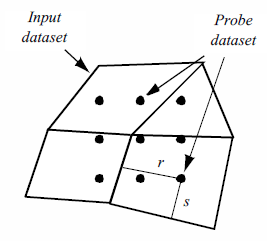
\includegraphics[width=0.96\linewidth]{Figure9-18b}
		\captionsetup{justification=centering}
		\caption{Probe interpolation}
		\label{fig:Figure9-18b}
	\end{subfigure}
	\caption{Probing. The geometry of one dataset \textit{(Probe)} is used to extract dataset attributes from anther dataset \textit{(Input)}.}\label{fig:Figure9-18}
\end{figure}

Figure \ref{fig:Figure9-18}(b) illustrates the details of the probing process. For every point in the probe dataset, the location in the input dataset (i.e., cell, subcell, and parametric coordinates) and interpolation weights are determined. Then the data values from the cell are interpolated to the probe point. Probe points that are outside the input dataset are assigned a nil (or appropriate) value. This process repeats for all points in the probe dataset.

Probing can be used to reduce data or to view data in a particular fashion.

\begin{itemize}

\item Data is reduced when the probe operation is limited to a subregion of the input dataset, or the number of probe points is less than the number of input points.

\item Data can be viewed in a particular fashion by sampling on specially selected datasets. Using a probe dataset consisting of a line enables x-y plotting along a line, or using a plane allows surface color mapping or line contouring.

\end{itemize}

Probing must be used carefully or errors may be introduced. Under-sampling data in a region can miss important high-frequency information or localized data variations. Oversampling data, while not creating error, can give false confidence in the accuracy of the data. Thus the sampling frequency should have a similar density as the input dataset, or if higher density, the visualization should be carefully annotated as to the original data frequency.

One important application of probing converts irregular or unstructured data to structured form using a volume of appropriate resolution as a probe to sample the unstructured data. This is useful if we use volume rendering or other volume visualization techniques to view our data.

\begin{figure}[!htb]
	\floatbox[{\capbeside\thisfloatsetup{capbesideposition={right,center},capbesidewidth=0.4\textwidth}}]{figure}[\FBwidth]
	{\caption{Probing data in a combustor.  Probes are regular arrays of $50^2$ points that are then passed through a contouring filter.(\href{https://lorensen.github.io/VTKExamples/site/Cxx/VisualizationAlgorithms/ProbeCombustor/}{ProbeCombustor.cxx} or \href{https://lorensen.github.io/VTKExamples/site/Python/VisualizationAlgorithms/ProbeCombustor/}{ProbeCombustor.py})}\label{fig:Figure9-19}}
	{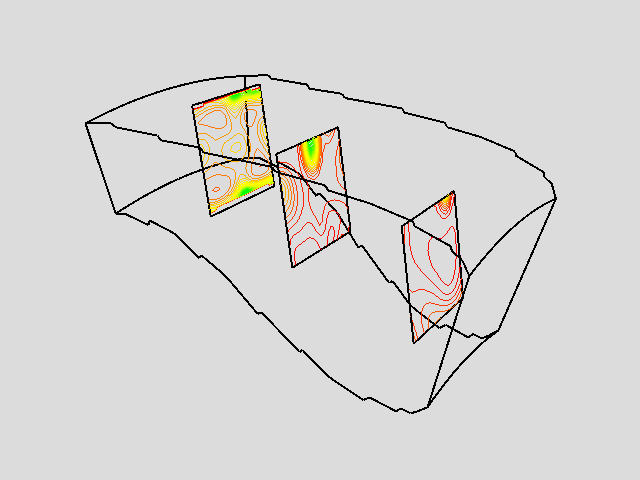
\includegraphics[width=0.6\textwidth]{Figure9-19}}
\end{figure}

Figure \ref{fig:Figure9-19} shows an example of three probes. The probes sample flow density in a structured grid. The output of the probes is passed through a contour filter to generate contour lines. As this figure illustrates, we can be selective with the location and extent of the probe, allowing us to focus on important regions in the data.

\subsection{Triangle Strip Generation}

Triangle strips are compact representations of triangle polygons as described in ``Triangle Strip'' on page \pageref{subsec:linear_cells.triangle_strip}. Many rendering libraries include triangle strips as graphics primitives because they are a high-performance alternative to general polygon rendering.

Visualization and graphics data is often represented with triangles. Marching cubes, for example, generates thousands and potentially millions of triangles to represent an isosurface. To achieve greater performance in our visualizations, we can convert triangle polygons into triangle strips. Or, if data is represented using polygons, we can first triangulate the polygons and then create triangle strips.

\begin{figure}[htb]
	\begin{subfigure}[h]{0.48\linewidth}
		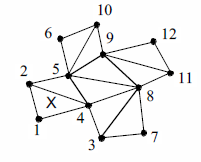
\includegraphics[width=0.96\linewidth]{Figure9-20a}
		\captionsetup{justification=centering}
		\caption*{Select first triangle}
		\label{fig:Figure9-20a}
	\end{subfigure}
	\hfill
	\begin{subfigure}[h]{0.48\linewidth}
		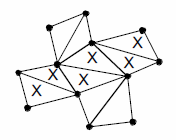
\includegraphics[width=0.96\linewidth]{Figure9-20b}
		\captionsetup{justification=centering}
		\caption*{Extend strip}
		\label{fig:Figure9-20b}
	\end{subfigure}
	\begin{subfigure}[h]{0.48\linewidth}
		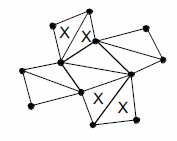
\includegraphics[width=0.96\linewidth]{Figure9-20c}
		\captionsetup{justification=centering}
		\caption*{Create additional strips}
		\label{fig:Figure9-20c}
	\end{subfigure}
	\hfill
	\begin{subfigure}[h]{0.48\linewidth}
    \centering
        \begin{minipage}[b]{.4\textwidth}
        \centering
        Representation:\\
        (1,2,4,5,8,9,11,12)\\
        (6,5,10,9)\\
        (4,3,8,7)
        \end{minipage}
		\captionsetup{justification=centering}
		\caption*{}
	\end{subfigure}
	\caption{Creating triangle strips.}\label{fig:Figure9-20}
\end{figure}


A simple method to generate triangle strips uses greedy gathering of triangles into a strip (Figure \ref{fig:Figure9-20}). The method proceeds as follows. An ``unmarked'' triangle is found to initialize the strip --- unmarked triangles are triangles that have not yet been gathered into a triangle strip. Starting with the initial triangle, the strip may grow in one of three directions, corresponding to the three edges of the triangle. We choose to grow the strip in the direction of the first unmarked neighbor triangle we encounter. If there are no unmarked neighbors the triangle strip is complete; otherwise, the strip is extended by adding triangles to the list that satisfy triangle strip topology. The strip is grown until no unmarked neighbor can be found. Additional strips are then created using the same procedure until every triangle is marked.

The length of the triangle strips varies greatly depending on the structure of the triangle mesh.

\begin{figure}[!htb]
	\centering
	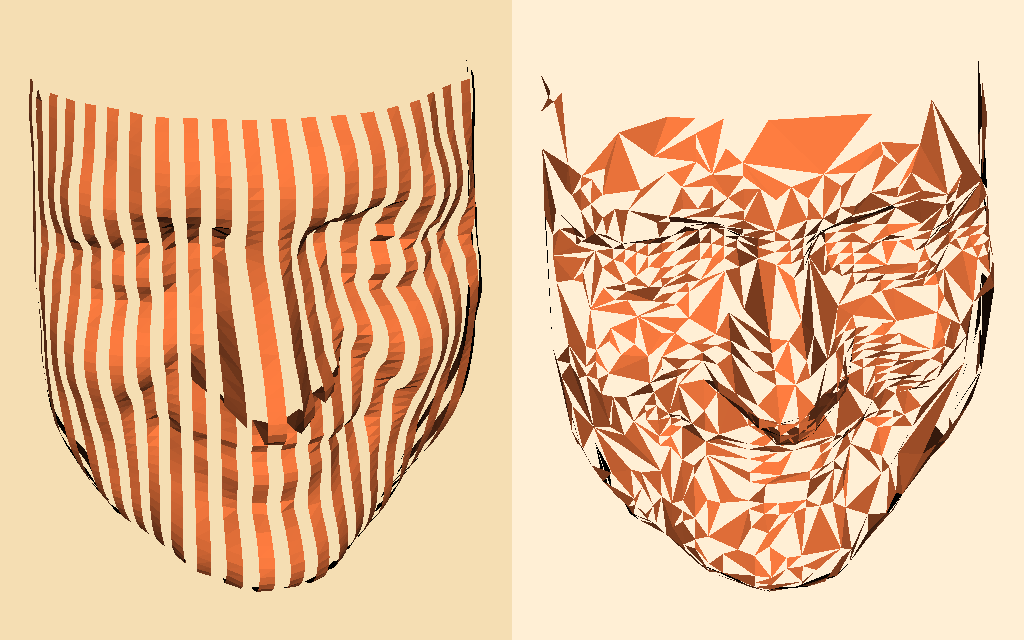
\includegraphics[width=0.98\textwidth]{Figure9-21}
	\caption{Triangle strip examples. Left, structured triangle mesh consisting of 134 strips each of 390 triangles. Right, Unstructured triangle mesh consisting of 2227 strips of average length 3.94, longest strip 101 triangles. Images are generated by displaying every other triangle strip.(\href{https://lorensen.github.io/VTKExamples/site/Cxx/Rendering/StripFran/}{StripFran.cxx} or \href{https://lorensen.github.io/VTKExamples/site/Python/Rendering/StripFran/}{StripFran.py})}
	\label{fig:Figure9-21}
\end{figure}


Figure \ref{fig:Figure9-21}(left) shows triangle strips each of 390 triangles in length from a dataset that was originally structured. Such a case is an exception: unstructured triangle meshes typically average about 5-6 triangles per strip (Figure \ref{fig:Figure9-21}(right)). Even so, the memory savings are impressive. A triangle strip of length 6 requires 8 points to represent, while 8 triangles require 24 points, for a memory savings of 66.7 percent. Rendering speed may be greatly affected, too, depending upon the capabilities of the rendering system.

\subsection{Connectivity}
\label{subsec:connectivity}

\begin{figure}[htb]
	\begin{subfigure}[h]{0.32\linewidth}
		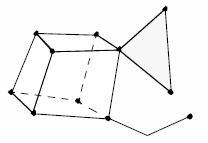
\includegraphics[width=0.96\linewidth]{Figure9-22a}
		\captionsetup{justification=centering}
		\caption*{Point connected}
		\label{fig:Figure9-22a}
	\end{subfigure}
	\hfill
	\begin{subfigure}[h]{0.32\linewidth}
		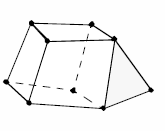
\includegraphics[width=0.96\linewidth]{Figure9-22b}
		\captionsetup{justification=centering}
		\caption*{Edge connected}
		\label{fig:Figure9-22b}
	\end{subfigure}
	\begin{subfigure}[h]{0.32\linewidth}
		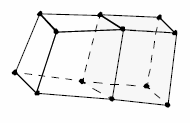
\includegraphics[width=0.96\linewidth]{Figure9-22c}
		\captionsetup{justification=centering}
		\caption*{Face connected}
		\label{fig:Figure9-22c}
	\end{subfigure}
	\caption{Connected cells.}\label{fig:Figure9-22}
\end{figure}

Intercell connectivity is a topological property of datasets. Cells are topologically connected when they share boundary features such as points, edges, or faces (Figure \ref{fig:Figure9-22}). Connectivity is useful in a number of modeling applications, particularly when we want to separate out ``parts'' of a dataset.

\begin{figure}[!htb]
	\centering
	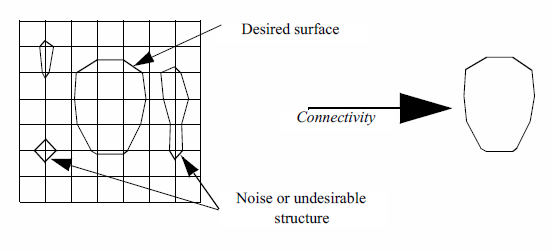
\includegraphics[width=0.98\textwidth]{Figure9-23}
	\caption{Extracting portion of isosurface of interest using connectivity.}
	\label{fig:Figure9-23}
\end{figure}

One application of connectivity extracts a meaningful portion of an isosurface. If the isosurface is generated from measured data such as an MRI or CT scan, it likely contains ``noise'' or unimportant anatomical structure. Using connectivity algorithms, we can separate out the part of the isosurface that we desire, either by eliminating noise or undesirable anatomical structure. Figure \ref{fig:Figure9-23} is an example where a 2D surface of interest (e.g., an isocontour) is extracted from a noisy signal.

Connectivity algorithms can be implemented using a recursive visit method. We begin by choosing an arbitrary cell and mark it ``visited''. Then, depending upon the type of connectivity desired (i.e., point, edge, face), we gather the appropriate neighbors and mark them visited. This process repeats recursively until all connected cells are visited. We generally refer to such a set of connected cells as a connected ``surface'' even though the cells may be of a topological dimension other than two.

To identify additional connected surfaces we locate another unvisited cell and repeat the processes described previously. We continue to identify connected surfaces until every cell in the dataset is visited. As each connected surface is identified, it is assigned a surface number. We can use this number to specify the surfaces to extract or we can specify ``seed'' points or cells and extract the surfaces connected to them.

In some cases the recursion depth of the connectivity algorithm becomes larger than the computer system can manage. In this case, we can specify a maximum recursion depth. When this depth is exceeded, recursion is terminated and the current cells in the recursion are used as seeds to restart the recursion.

\subsubsection{Hybrid Techniques}

Recent work has focused on combining triangulation and basis function techniques for interpolating 2D bivariate data. The basic idea is as follows. A triangulation of P is constructed. Then an interpolating network of curves is defined over the edges of the triangulation. These curves are constructed with certain minimization properties of interpolating splines. Finally, the curve network is used to construct a series of triangular basis functions, or surface patches, that exhibit continuity in function value, and possibly higher order derivatives. (See \cite{Nielson91a} for more information.)

\subsection{Polygon Normal Generation}

\begin{figure}[htb]
    \centering
	\begin{subfigure}[h]{0.96\linewidth}
		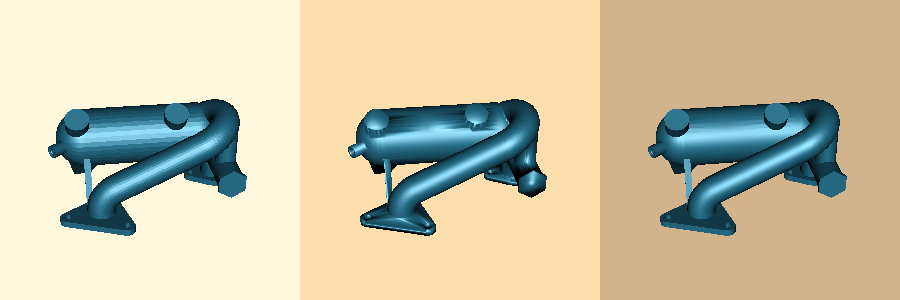
\includegraphics[width=0.96\linewidth]{Figure9-24a}
		\captionsetup{justification=centering}
		\caption{Original faceted model (left), Naive normal generation,(center), Split-edge normal generation(right) (\href{https://lorensen.github.io/VTKExamples/site/Cxx/Visualization/NormalsDemo/}{NormalsDemo.cxx} or \href{https://lorensen.github.io/VTKExamples/site/Python/Visualization/NormalsDemo/}{NormalsDemo.py})}
		\label{fig:Figure9-24a}
	\end{subfigure}
	\hfill
	\begin{subfigure}[h]{0.4\linewidth}
		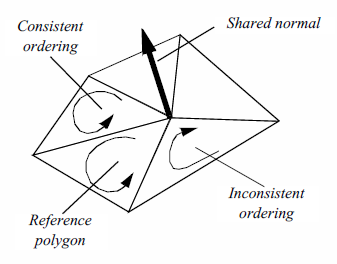
\includegraphics[width=0.96\linewidth]{Figure9-24b}
		\captionsetup{justification=centering}
		\caption{Normal computation}
		\label{fig:Figure9-24b}
	\end{subfigure}
	\caption{ Surface normal generation. Left -- faceted model without normals. Center -- sharp edges are poorly represented using shared normals as shown on the corners of this model. Right -- normal generation with sharp edges split.}\label{fig:Figure9-24}
\end{figure}

Gouraud and Phong shading (see page \pageref{subsection:rasterization.phong}) can improve the appearance of rendered polygons. Both techniques require point normals. Unfortunately polygonal meshes do not always contain point normals, or data file formats may not support point normals. Examples include the marching cubes algorithm for general datasets (which typically will not generate surface normals) and the stereo lithography file format (does not support point normals). Figure \ref{fig:Figure9-24a}(left) shows a model defined from stereo-lithography format. The faceting of the model is clearly evident.

To address this situation we can compute surface normals from the polygonal mesh. A simple approach follows. First, polygon normals are computed around a common point. These normals are then averaged at the point, and the normal is renormalized (i.e., $\vert n \vert = 1$ ) and associated with the point. This approach works well under two conditions.

\begin{enumerate}

\item The orientation of all polygons surrounding the point are consistent as shown in Figure \ref{fig:Figure9-24b}. A polygon is oriented consistently if the order of defining polygon points is consistent with its edge neighbors. That is, if polygon $p$ is defined by points $(1,2,3)$, then the polygon edge neighbor $p_{23}$ must use the edge $(2,3)$ in the direction $(3,2)$. If not consistent, then the average point normal may be zero or not accurately represent the orientation of the surface. This is because the polygon normal is computed from a cross product of the edges formed by its defining points.

\item The angular difference in surface normals between adjacent polygons is small. Otherwise, sharp corners or edges will have a washed out appearance when rendered, resulting in an unsatisfactory image (Figure \ref{fig:Figure9-24a}(center)).

\end{enumerate}

To avoid these problems we adopt a more complex polygon normal generation algorithm. This approach includes steps to insure that polygons are oriented consistently, and an edge-splitting scheme that duplicates points across sharp edges.

To orient edges consistently we use a recursive neighbor traversal. An initial polygon is selected and marked ``consistent''. For each edge neighbor of the initial polygon, the ordering of the neighbor polygon points is checked --- if not consistent, the ordering is reversed. The neighbor polygon is then marked ``consistent''. This process repeats recursively for each edge neighbor until all neighbors are marked ``consistent''. In some cases there may be more than one connected surface, so that the process may have to be repeated until all polygons are visited.

\begin{figure}[htb]
    \centering
	\begin{subfigure}[h]{0.48\linewidth}
		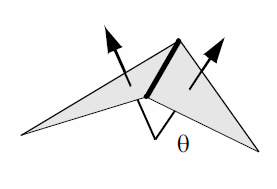
\includegraphics[width=0.96\linewidth]{Figure9-25a}
		\captionsetup{justification=centering}
		\caption{Feature edge}
		\label{fig:Figure9-25a}
	\end{subfigure}
	\hfill
	\begin{subfigure}[h]{0.48\linewidth}
		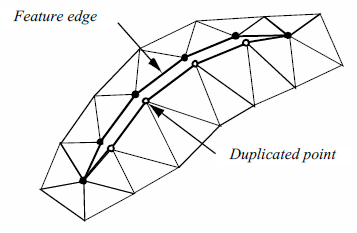
\includegraphics[width=0.96\linewidth]{Figure9-25b}
		\captionsetup{justification=centering}
		\caption{Exaggerated splitting of feature edge}
		\label{fig:Figure9-25b}
	\end{subfigure}
	\caption{Computing feature angles (a) and splitting edges (b).}\label{fig:Figure9-25}
\end{figure}

A similar traversal method splits sharp edges. A sharp edge is an edge shared by two polygons whose normals vary by a user-specified feature angle. The feature angle between two polygons is the angle between their normals (Figure \ref{fig:Figure9-25a}). When sharp edges are encountered during the recursive traversal, the points along the edge are duplicated, effectively disconnecting the mesh along that edge (Figure \ref{fig:Figure9-25b}). Then, when shared polygon normals are computed later in the process, contributions to the average normal across sharp edges is prevented.

On some computers limitations on recursion depth may become a problem. Polygonal surfaces can consist of millions of polygons, resulting in large recursion depth. As a result, the depth of recursion can be specified by the user. If recursion depth exceeds the specified value, the recursion halts and the polygons on the boundary of the recursion become seeds to begin the process again.

Figure \ref{fig:Figure9-24a}(right) shows the result of the advanced normal generation technique with a feature angle of 60$^\circ$. Sharp edges are well defined and curved areas lack the faceting evident in the original model. The figure is shown with Gouraud shading.

\subsection{Decimation}

\begin{figure}[!htb]
	\centering
	\includegraphics[width=0.98\textwidth]{Figure9-26}
	\caption{Overview of decimation algorithm.}
	\label{fig:Figure9-26}
\end{figure}

Various data compression techniques have been developed in response to large data size. The UNIX utilities \texttt{compress/uncompress} and the PC utility \texttt{zip} compress data files. The MPEG compression algorithm compresses video sequences. These techniques may be lossless, meaning that no data is lost between the compression/decompression steps, or lossy, meaning that data is lost during compression. The utilities \texttt{compress/uncompress} and \texttt{zip} are loss-less, while MPEG is lossy.

In graphics, data compression techniques have been developed as well. The subsampling methods we saw earlier in this chapter are an example of simple data compression techniques for visualization data. Another emerging area of graphics data compression is polygon reduction techniques.

Polygon reduction techniques reduce the number of polygons required to model an object. The size of models, in terms of polygon count, has grown tremendously over the last few years. This is because many models are created using digital measuring devices such as laser scanners or satellites. These devices can generate data at tremendous rates. For example, a laser digitizer can generate on the order of 500,000 triangles in a 15--second scan. Visualization algorithms such as marching cubes also generate large numbers of polygons: one to three million triangles from a $512^3$ volume is typical.

One polygon reduction technique is the decimation algorithm \cite{Schroeder92a}. The goal of the decimation algorithm is to reduce the total number of triangles in a triangle mesh, preserving the original topology and forming a good approximation to the original geometry. A triangle mesh is a special form of a polygonal mesh, where each polygon is a triangle. If need be, a polygon mesh can be converted to a triangle mesh using standard polygon triangulation methods.

Decimation is related to the subsampling technique for unstructured meshes described in Figure \ref{fig:Figure9-17b}. The differences are that

\begin{itemize}

\item decimation treats only triangle meshes not arbitrary unstructured grids;

\item the choice of which points to delete is a function of a decimation criterion, a measure of the local error introduced by deleting a point; and

\item the triangulation of the hole created by deleting the point is carried out in a way as to preserve edges or other important features.

\end{itemize}

Decimation proceeds by iteratively visiting each point in a triangle mesh. For each point, three basic steps are carried out (Figure \ref{fig:Figure9-26}). The first step classifies the local geometry and topology in the neighborhood of the point. The classification yields one of the five categories shown in the figure: simple, boundary, complex, edge, and corner point. Based on this classification, the second step uses a local error measure (i.e., the decimation criterion) to determine whether the point can be deleted. If the criterion is satisfied, the third step deletes the point (along with associated triangles), and triangulates the resulting hole. A more detailed description of each of these steps and example applications follow.

\begin{description}

\item[Point Classification.] The first step of the decimation algorithm characterizes the local geometry and topology for a given point. The outcome of classification determines whether the vertex is a potential candidate for deletion, and if it is, which criteria to use.

Each point may be assigned one of five possible classifications: simple, complex, boundary, interior edge, or corner vertex. Examples of each type are shown in Figure \ref{fig:Figure9-26}.

A \emph{simple point} is surrounded by a complete cycle of triangles, and each edge that uses the point is used by exactly two triangles. If the edge is not used by two triangles, or if the point is used by a triangle not in the cycle of triangles, then the point is \emph{complex}. These are nonmanifold cases.

A point that is on the boundary of a mesh, that is, within a semicycle of triangles, is a \emph{boundary point}.

A \emph{simple point} can be further classified as an \emph{interior edge} or \emph{corner point}. These classifications are based on the local mesh geometry. If the surface normal angle between two adjacent triangles is greater than a specified \emph{feature angle}, then a \emph{feature edge} exists (see Figure \ref{fig:Figure9-25a}). When a point is used by two feature edges, the point is an interior edge point. If one, three, or more feature edges use the point, the point is a \emph{corner point}.

Complex and corner vertices are not deleted from the triangle mesh; all other vertices become candidates for deletion.

\item[Decimation Criterion.] Once we have a candidate point for deletion, we estimate the error that would result by deleting the point and then replacing it (and its associated triangles) with another triangulation. There are a number of possible error measures; but the simplest are based on distance measures of local planarity or local colinearity (Figure \ref{fig:Figure9-26}).

In the local region surrounding a simple point, the mesh is considered nearly ``flat'', since there are by definition no feature edges. Hence, simple points use an error measure based on distance to plane. The plane passing through the local region can be computed either using a leastsquares plane or by computing an area-averaged plane.

Points classified as boundary or interior edge are considered to lay on an edge, and use a distance to edge error measure. That is, we compute the distance that the candidate point is from the new edge formed during the triangulation process.

A point satisfies the decimation criterion \emph{d} if its distance measure is less than \emph{d}. The point can then be deleted. All triangles using the point are deleted as well, leaving a ``hole'' in the mesh. This hole is patched using a local triangulation process.

\item[Triangulation.] \label{subsec:decimation.triangulation} After deleting a point, the resulting hole must be retriangulated. Although the hole, defined by a loop of edges, is topologically two dimensional, it is generally non-planar, and therefore general purpose 2D triangulation techniques cannot be used. Instead, we use a special recursive 3D divide-and-conquer technique to triangulate the loop.

Triangulation proceeds as follows. An initial split plane is chosen to divide the loop in half and create two subloops. If all the points in each subloop lie on opposite sides of the plane, then the split is a valid one. In addition, an aspect ratio check insures that the loop is not too long and skinny, thereby resulting in needle-like triangles. The aspect ratio is the ratio between the length of the split line to the minimum distance of a point in the subloop to the split plane. If the candidate split plane is not valid or does not satisfy the aspect ratio criterion, then another candidate split plane is evaluated. Once a split plane is found, then the subdivision of each subloop continues recursively until a subloop consists of three edges. In this case, the subloop generates a triangle and halts the recursion.

Occasionally, triangulation fails because no split plane can be found. In this case, the candidate point is not deleted and the mesh is left in its original state. This poses no problem to the algorithm and decimation continues by visiting the next point in the dataset.

\item[Results.] Typical compression rates for the decimation algorithm range from 2:1 to 100:1, with 10:1 a nominal figure for `large` (i.e., $10^5$ triangles) datasets. The results vary greatly depending upon the type of data. CAD models typically reduce the least because these models have many sharp  edges and other detailed features, and the CAD modellers usually produce minimal triangulations. Terrain data, especially if relatively flat regions are present, may reduce at rates of 100:1.

\begin{figure}[htb]
    \centering
	\begin{subfigure}[h]{0.96\linewidth}
		\includegraphics[width=0.96\linewidth]{Figure9-27a}
		\captionsetup{justification=centering}
		\caption{Decimation of laser digitizer data (\href{https://lorensen.github.io/VTKExamples/site/Cxx/VisualizationAlgorithms/DecimateFran/}{DecimateFran.cxx} or \href{https://lorensen.github.io/VTKExamples/site/Python/VisualizationAlgorithms/DecimateFran/}{DecimateFran.py})}
		\label{fig:Figure9-27a}
	\end{subfigure}
	\hfill
	\begin{subfigure}[h]{0.96\linewidth}
		\includegraphics[width=0.96\linewidth]{Figure9-27b}
		\captionsetup{justification=centering}
		\caption{Decimation of laser digitizer data (\href{https://lorensen.github.io/VTKExamples/site/Cxx/VisualizationAlgorithms/DecimateHawaii/}{DecimateHawaii.cxx} or \href{https://lorensen.github.io/VTKExamples/site/Python/VisualizationAlgorithms/DecimateHawaii/}{DecimateHawaii.py})}
		\label{fig:Figure9-27b}
	\end{subfigure}
	\caption{Examples of decimation algorithm. Triangle meshes are shown in wireframe.}\label{fig:Figure9-27}
\end{figure}

Figure \ref{fig:Figure9-27} shows two applications of decimation to laser digitized data and to a terrain model of Honolulu, Hawaii. In both cases the reduction was on the order of 90 percent for a 10:1 compression ratio. Wireframe images are shown to accentuate the density of the polygonal meshes. The left-hand image in each pair is the original data; the right-hand image is the decimated mesh.

Notice the gradations in the decimated mesh around features of high curvature. The advantage of decimation, as compared to subsampling techniques, is that the mesh is adaptively modified to retain more details in areas of high curvature.

\item[Advanced Techniques.] Polygon reduction is an active field of research. Many powerful algorithms beyond the decimation algorithm have been presented (see ``Bibliographic Notes'' on page  \pageref{sec:bibliographic_notes.ch09}) in this Chapter). Although we cannot cover the field in its entirety in this section, there are two notable trends worth addressing. First, progressive schemes \cite{Hoppe96} allow incremental transmission and reconstruction of triangle meshes --- this is especially important for Web-based geometry visualization. Second, recent algorithms modify the topology of the mesh \cite{He96} \cite{Popovic97} \cite{Schroeder97}. This feature is essential towards obtaining arbitrary levels of mesh reduction.

A \emph{progressive mesh} is a series of triangle meshes $M_i$i related by the operations

\begin{equation}\label{eq:9.14}
\left(\hat{M} = M^n \right) \to M^{n - 1} \to \ldots \to M^1 \to M^0
\end{equation}
\myequations{Progressive mesh operations.}

where $\vec{M}$ and $M^n$ represent the mesh at full resolution, and $M^0$ is a simplified base mesh. The critical characteristic of progressive meshes is that is possible to choose the mesh operations in such a way to make them invertible. Then the operations can be applied in reverse order (starting with the base mesh $M^0$)

\begin{equation}\label{eq:9.15}
M^0 \to M^1 \to \ldots \to M^{n - 1} \to M^n
\end{equation}
\myequations{Progressive mesh operations (reverse order).}

to obtain a mesh of desired reduction level (assuming that the reduction level is less than the base mesh $M^0$).

\begin{figure}[htb]
    \centering
	\begin{subfigure}[h]{0.96\linewidth}
		\includegraphics[width=0.96\linewidth]{Figure9-28a}
		\captionsetup{justification=centering}
		\caption{A edge collapse and split}
		\label{fig:Figure9-28a}
	\end{subfigure}
	\hfill
	\begin{subfigure}[h]{0.96\linewidth}
		\includegraphics[width=0.96\linewidth]{Figure9-28b}
		\captionsetup{justification=centering}
		\caption{A vertex split and merge}
		\label{fig:Figure9-28b}
	\end{subfigure}
	\hfill
	\begin{subfigure}[h]{0.96\linewidth}
		\includegraphics[width=0.96\linewidth]{Figure9-28c}
		\captionsetup{justification=centering}
        \caption{Vertex splits applied to various features. Darker lines indicate feature edges.}
		\label{fig:Figure9-28c}
	\end{subfigure}
	\caption{Examples of decimation algorithm. Triangle meshes are shown in wireframe.}\label{fig:Figure9-28}
\end{figure}

One such invertible operator is an edge collapse and its inverse is the edge split shown in Figure \ref{fig:Figure9-28a}). Each collapse of an interior mesh edge results in the elimination of two triangles (or one triangle if the collapsed vertex is on a boundary). The operation is represented by five values

\begin{equation}\label{eq:9.16}
\text{Edge Collapse/Split}(v_s, v_t, v_\ell, v_r, A)
\end{equation}
\myequations{Edge collapse/split.}

where $v_s$ is the vertex to collapse/split, $v_t$ is the vertex being collapsed to / split from, and $v_l$ and $v_r$ are two additional vertices to the left and right of the split edge. These two vertices in conjunction with $v_s$ and $v_t$ define the two triangles deleted or added. A represents vertex attribute information, which at a minimum contains the coordinates x of the collapsed / split vertex $v_s$. (Note: in the context of the decimation algorithm, the edge collapse operator replaces the recursive triangulation process.)

While progressive meshes allow us to compactly store and transmit triangle meshes, the problem remains that the size of the base mesh is often larger than desired reduction level. Since in some applications we wish to realize any given level, we want the base mesh to contain no triangles

\begin{equation}\label{eq:9.17}
\left(\hat{M} = M^n \right) \to M^{n - 1} \to \ldots \to M^1 \to \left(M^0 = M(V, \varnothing)\right)
\end{equation}
\myequations{Edge collapse/split.}

(some vertices are necessary to initiate the edge split operations). To address this problem, the invertible edge collapse/split operator --- which is topology preserving --- is extended with a vertex split/merge operator. The vertex split/merge operator modifies the topology of the mesh and allows arbitrary levels of reduction.

A mesh split occurs when we replace vertex $v_s$ with vertex $v_t$ in the connectivity list of one or more triangles that originally used vertex $v_s$ (Figure \ref{fig:Figure9-28b}). The new vertex $v_t$ is given exactly the same coordinate value as vs. Splits introduce a ``crack'' or ``hole'' into the mesh. We prefer not to split the mesh, but at high decimation rates this relieves topological constraint and enables further decimation. Splitting is only invoked when a valid edge collapse is not available, or when a vertex cannot be triangulated (e.g., a nonmanifold vertex). Once the split operation occurs, the vertices $v_s$ and $v_t$ are re-inserted into the priority queue.

Different splitting strategies are used depending on the classification of the vertex (Figure \ref{fig:Figure9-28c}). Interior edge vertices are split along the feature edges, as are corner vertices.

Nonmanifold vertices are split into separate manifold pieces. In any other type of vertex splitting occurs by arbitrarily separating the loop into two pieces. For example, if a simple vertex cannot be deleted because a valid edge collapse is not available, the loop of triangles will be arbitrarily divided in half (possibly in a recursive process).

Like the edge collapse/split, the vertex split/merge can also be represented as a compact operation. A vertex split/merge operation can be represented with four values

\begin{equation}\label{eq:9.18}
\text{Vertex Split/Merge}(v_s, v_t, v_l, v_r)
\end{equation}
\myequations{Vertex split/merge.}

The vertices $v_l$ and $v_r$ define a sweep of triangles (from $v_r$ to $v_l$ ) that are to be separated from the original vertex vs (we adopt a counter--clockwise ordering convention to uniquely define the sweep of triangles).

\begin{figure}[htb]
    \centering
	\begin{subfigure}[h]{0.32\linewidth}
		\includegraphics[width=0.96\linewidth]{Figure9-29a}
		\captionsetup{justification=centering}
		\caption{Original model \\ 2,624 triangles}
		\label{fig:Figure9-29a}
	\end{subfigure}
	\hfill
	\begin{subfigure}[h]{0.32\linewidth}
		\includegraphics[width=0.96\linewidth]{Figure9-29b}
		\captionsetup{justification=centering}
		\caption{Shortly after splitting \\ 157 triangles}
		\label{fig:Figure9-29b}
	\end{subfigure}
	\hfill
	\begin{subfigure}[h]{0.32\linewidth}
		\includegraphics[width=0.96\linewidth]{Figure9-29c}
		\captionsetup{justification=centering}
        \caption{Final model \\ 4 triangles.}
		\label{fig:Figure9-29c}
	\end{subfigure}
	\hfill
	\begin{subfigure}[h]{0.32\linewidth}
		\includegraphics[width=0.96\linewidth]{Figure9-29d}
		\captionsetup{justification=centering}
		\caption{Original model \\ 11,006 triangles}
		\label{fig:Figure9-29d}
	\end{subfigure}
	\hfill
	\begin{subfigure}[h]{0.32\linewidth}
		\includegraphics[width=0.96\linewidth]{Figure9-29e}
		\captionsetup{justification=centering}
		\caption{Reduction 50\% \\ 5518 triangles}
		\label{fig:Figure9-29e}
	\end{subfigure}
	\hfill
	\begin{subfigure}[h]{0.32\linewidth}
		\includegraphics[width=0.96\linewidth]{Figure9-29f}
		\captionsetup{justification=centering}
        \caption{Reduction 98\% \\ 220 triangles}
		\label{fig:Figure9-29f}
	\end{subfigure}
	\caption{ Results of topology modifying progressive mesh algorithm.}\label{fig:Figure9-29}
\end{figure}

Figure \ref{fig:Figure9-29} shows the results of applying the topology modifying progressive mesh algorithm to two sets of data. In Figure \ref{fig:Figure9-29}(a-c), a thin plate with holes is decimated (the darker lines show split edges). The middle image in the sequence shows the limits of topology on the algorithm. It is only when the topology of the mesh is allowed to be modified that the final level of reduction is possible. Figure \ref{fig:Figure9-29}(d-f) shows the same algorithm applied to CAD data.

\end{description}

\clearpage

\subsection{Mesh Smoothing}
\label{subsec:mesh_smoothing}

Mesh smoothing is a technique that adjusts the point coordinates of a dataset. The purpose of mesh smoothing is to improve the appearance of a mesh, and/or improve the shape of dataset cells. During smoothing the topology of the dataset is not modified, only the geometry. Applications of mesh smoothing include improving the appearance of isosurfaces, or as a modelling tool to remove surface noise. The appearance of models can be dramatically improved by applying mesh smoothing. Figure \ref{fig:Figure9-30} is an example of smoothing applied to analytic surface (a semicylinder) with a random surface distortion (\texttt{smoothCyl.tcl}).

\begin{figure}[!htb]
	\centering
	\includegraphics[width=0.98\textwidth]{Figure9-30}
	\caption{Mesh smoothing applied to a semicylinder. Lower left image is the original model. On the \emph{x}--axis the number of smoothing iterations is modified. On the  \emph{y}--axis the relaxation factor is modified.}
	\label{fig:Figure9-30}
\end{figure}

A simple, yet effective technique is Laplacian smoothing. The Laplacian smoothing equation for a point $p_i$ at position $x_i$ is given by

\begin{equation}\label{eq:9.19}
\overrightarrow{x\ }_{i+1} = \overrightarrow{x\ }_i + \lambda \overrightarrow{V\ }(i, j) = \overrightarrow{x\ }_i + \lambda \sum_{j = 0}^{n}\overrightarrow{x\ }_j - \overrightarrow{x\ }_i
\end{equation}
\myequations{Laplacian smoothing.}

where $x_i + 1$ is the new coordinate position, and $x_j$ are the positions of points $p_j$ ``connected'' to $p_i$, and $\lambda$ is a user-specified weight. Geometrically this relation is depicted in Figure \ref{fig:Figure9-31a}. Here the vertex $p_i$ is connected to the surrounding points $p_j$ via edges. The equation expresses that the new position $x_i + 1$ is offset from the original position $x_i$ plus the average vector $\overrightarrow{V\ }_{ij}$ multiplied by $\lambda$. Typically, the factor $\lambda$ is a small number (e.g., 0.01), and the process is executed repeatedly (e.g., 50-100 iterations). Notice that the overall effect of smoothing is to reduce the high frequency surface information. The algorithm will reduce surface curvature and tend to flatten the surface.

\begin{figure}[!htb]
    \thisfloatsetup{capbesideposition={right,center},capbesidewidth=0.32\textwidth}
    \fcapside[\FBwidth]
    {%
      \begin{subfloatrow}
        \ffigbox[0.32\textwidth]{\caption{}\label{fig:Figure9-31a}
          \centering
          \includegraphics[width=\linewidth]{Figure9-31a}}{}
        \ffigbox[0.32\textwidth]{\caption{}\label{fig:Figure9-31b}
          \centering
          \includegraphics[width=\linewidth]{Figure9-31b}}{}
      \end{subfloatrow}
    }{\caption {Mesh smoothing. (a) Motion of point. (b) Smoothing a point on an edge. Bold lines indicate connectivity.\label{fig:Figure9-31}}}
\end{figure}


Besides adjusting the number of iterations and smoothing factor, smoothing can be controlled by modifying the connections between $p_i$ and its surrounding points $p_j$. For example, if $p_i$ lies along a fold or sharp edge in the mesh, we may want to only use the two edge end points to compute the smoothing vector $\overrightarrow{V}_{ij}$, limiting the motion of $p_i$ along the edge (Figure \ref{fig:Figure9-31b}). We can also anchor $p_i$ to prevent any motion. Anchoring is useful for points that are located on ``corners'' or other special features such as nonmanifold attachments. One benefit of anchoring and controlling point connectivity is that we can limit the amount of shrinkage in the mesh. It also tends to produce better overall results. (In Figure \ref{fig:Figure9-30} the boundary points of the surface are constrained to move along the boundary, while the points at sharp corners are anchored.)

Although Laplacian smoothing works well in most cases, there are applications of Laplacian smoothing that can badly damage the mesh. Large numbers of smoothing iterations, or large smoothing factors, can cause excessive shrinkage and surface distortion. Some objects, like spheres or the cylinder shown in Figure \ref{fig:Figure9-30}, will lose volume with each iteration, and can even shrink to a point. In rare cases it is possible for the mesh to pull itself ``inside-out''. Situations like this occur when the average vector moves $p_i$ across a mesh boundary, causing some of the attached triangles to overlap or intersect.

Mesh smoothing is particularly useful when creating models that do not require high accuracy. As we have seen, smoothing modifies point coordinates and, therefore, surface geometry. Use smoothing to improve the appearance of models, but characterize error carefully if you are going to measure from a smoothed surface. Alternatively, you may want to design your own smoothing algorithms that better fit the underlying data.

\clearpage

\subsection{Swept Volumes and Surfaces}

Consider moving an object (e.g., your hand) over some path (e.g., raise your hand). How can we visualize this motion? The obvious answer is to form a time-animation sequence as the hand is moved. But what if we wish to statically represent the motion as well as the space that is traversed by the hand? Then we can use swept surfaces and swept volumes.

A swept volume is the volume of space occupied by an object as it moves through space along an arbitrary trajectory. A swept surface is the surface of the swept volume. Together, swept volumes and swept surfaces can statically represent the motion of objects.

Past efforts at creating swept surfaces and volumes have focused on analytical techniques. The mathematical representation of various 3D geometric primitives (e.g., lines, polygons, splines) was extended to include a fourth dimension of time (the path). Unfortunately, these approaches have never been practically successful, partly due to mathematical complexity and partly due to problem degeneracies.

Degeneracies occur when an n-dimensional object moves in such a way that its representation becomes (n-1)-dimensional. For example, moving a plane in the direction of its normal, sweeps out a 3D ``cubical'' volume. Sweeping the plane in a direction perpendicular to its normal, however, results in a degenerate condition, since the plane sweeps out a 2D ``rectangle''.

Instead of creating swept surfaces analytically, numerical approximation techniques can be used \cite{Schroeder94}. Implicit modeling provides the basis for an effective technique to visualize object motion via swept surfaces and volumes. The technique is immune to degeneracies and can treat any geometric representation for which a distance function can be computed, such as the VTK cell types.

\begin{figure}[htb]
    \centering
	\begin{subfigure}[h]{0.48\linewidth}
		\includegraphics[width=0.96\linewidth]{Figure9-32a}
		\captionsetup{justification=centering}
		\caption{Generate implicit model, $V_I$}
		\label{fig:Figure9-32a}
	\end{subfigure}
	\hfill
	\begin{subfigure}[h]{0.48\linewidth}
		\includegraphics[width=0.96\linewidth]{Figure9-32b}
		\captionsetup{justification=centering}
		\caption{Sweep implicit model through workspace volume, $V_W$}
		\label{fig:Figure9-32b}
	\end{subfigure}
	\hfill
	\begin{subfigure}[h]{0.48\linewidth}
		\includegraphics[width=0.96\linewidth]{Figure9-32c}
		\captionsetup{justification=centering}
        \caption{Generate swept surface via isosurface extraction. Use connectivity to extract single surface.}
		\label{fig:Figure9-32c}
	\end{subfigure}
	\caption{Overview of swept surface technique.}\label{fig:Figure9-32}
\end{figure}

The technique to generate swept surfaces and volumes using an implicit modeling approach proceeds as follows. The geometric model, or part, and a path describing the parts motion, or sweep trajectory ST, must be defined. Then we use the following steps as depicted in Figure \ref{fig:Figure9-32}.

\begin{enumerate}

\item Generate an implicit model from the part. This results in an implicit representation in the form of a volume. We call this the implicit model $V_I$.

\item Construct another volume, the workspace volume $V_W$, that strictly bounds $V_I$ as it moves along the path ST. Then sweep $V_I$ through $V_W$ by moving in small steps, $\delta x$, along ST. At each step, $s$, sample $V_I$ with the workspace volume $V_W$. We use a boolean union operation to perform the sampling.

\item Extract isosurface, or offset surface(s) from $V_W$ using a contouring algorithm such as marching cubes.

\item Step 3 may create multiple connected surfaces. If a single surface is desired, use connectivity to extract the single ``largest'' surface (in terms of number of triangles). This surface is an approximation to the swept surface, and the volume it encloses is an approximation to the swept volume.

\end{enumerate}

\begin{figure}[htb]
    \centering
	\begin{subfigure}[h]{0.48\linewidth}
		\includegraphics[width=0.96\linewidth]{Figure9-33a}
		\captionsetup{justification=centering}
		\caption{Inverse transform, $V_W$}
		\label{fig:Figure9-33a}
	\end{subfigure}
	\hfill
	\begin{subfigure}[h]{0.48\linewidth}
		\includegraphics[width=0.96\linewidth]{Figure9-33b}
		\captionsetup{justification=centering}
		\caption{Sample, $V_W$}
		\label{fig:Figure9-33b}
	\end{subfigure}
	\caption{Generating workspace volume by sampling implicit volume.}\label{fig:Figure9-33}
\end{figure}

There are a few points that require additional explanation. This algorithm uses two volumes, the implicit model and the workspace volume. Both are implicit models, but the workspace volume is used to accumulate the part as it moves along the sweep trajectory. In theory, the part could be sampled directly into the workspace volume to create the implicit model of the swept surface. Performance issues dictate that the implicit model is sampled into the workspace volume. This is because it is much faster to sample the implicit model of the part rather than the part itself, since computing the distance function from a part that may consist of tens of thousands of cells is relatively time consuming, compared to sampling the implicit model $V_I$.

Sampling $V_I$ is depicted in Figure \ref{fig:Figure9-33}. The sweep trajectory is defined by a series of transformation matrices $ST = {t_1, t_2,..., t_m}$. As the part moves along ST, interpolation is used to compute an inbetween transformation matrix t. Sampling is achieved by inverse transforming VW into the local space of $V_I$ using $t$. Then, similar to the probe operation described in ``Probing'' on page \pageref{subsec:probing}, the points of $V_W$ are transformed by the inverse of the transformation matrix $t^{-1}$, and used to interpolate the distance values from the implicit model $V_I$.

\begin{figure}[htb]
    \centering
	\begin{subfigure}[h]{0.48\linewidth}
		\includegraphics[width=0.96\linewidth]{Figure9-34a}
		\captionsetup{justification=centering}
		\caption{Inverse transform, $V_W$}
		\label{fig:Figure9-34a}
	\end{subfigure}
	\hfill
	\begin{subfigure}[h]{0.48\linewidth}
		\includegraphics[width=0.96\linewidth]{Figure9-34b}
		\captionsetup{justification=centering}
		\caption{Sample, $V_W$}
		\label{fig:Figure9-34b}
	\end{subfigure}
	\caption{Computing sampling and stepping error.}\label{fig:Figure9-34}
\end{figure}

Because we are dealing with an implicit modeling technique, parts with concave features can generate multiple surfaces. As discussed in ``Connectivity'' on page \pageref{subsec:connectivity} in this Chapter, the connectivity algorithm is used to separate out the swept surface. This final surface is an approximation to the actual swept surface, since we are sampling the actual geometric representation on an array of points (i.e., the implicit model), and then sampling the implicit model on another volume (i.e., the workspace volume). Also, stepping along the sweep trajectory generates errors proportional to the step size $\delta$x.

These errors can be characterized as follows (Figure \ref{fig:Figure9-34}). Given a voxel size $L/D$, where $L$ is the edge length of the volume, and $D$ is the dimension of the volume (assumed uniform for convenience), the maximum sampling error is

\begin{equation}\label{eq:9.20}
e \leq \dfrac{\sqrt{3}}{2} \dfrac{L}{D}
\end{equation}
\myequations{Maximum sampling error.}

The error due to stepping, which includes both translation and rotational components, is bounded by $\delta x / 2$, where $\delta x$ is the maximum displacement of any point on the implicit model at any given translational step. Combining these terms for sampling both volumes and the error due to stepping, the total error is

\begin{equation}\label{eq:9.21}
e_\text{tot} \leq \dfrac{\sqrt{3}}{2}\left( \dfrac{L_\text{I}}{D_\text{I}}
  + \dfrac{L_\text{W}}{D_\text{W}}\right) + \dfrac{\Delta x}{2}
\end{equation}
\myequations{Total error.}

\noindent where the subscripts $I$ and $W$ refer to the implicit model and workspace volume, respectively.

\begin{figure}[htb]
    \centering
	\begin{subfigure}[h]{0.48\linewidth}
		\includegraphics[width=0.96\linewidth]{Figure9-35a}
		\captionsetup{justification=centering}
		\caption{Translated and rotated mace}
		\label{fig:Figure9-35a}
	\end{subfigure}
	\hfill
	\begin{subfigure}[h]{0.48\linewidth}
		\includegraphics[width=0.96\linewidth]{Figure9-35b}
		\captionsetup{justification=centering}
		\caption{Line stroked ``vtk``}
		\label{fig:Figure9-35b}
	\end{subfigure}
	\caption{Swept surfaces. (a) Swept mace sampled at 25 locations. (b) Swept vtk sampled at 21 locations.}\label{fig:Figure9-35}
\end{figure}

To show the application of this algorithm, we have generated swept surfaces for the letters ``VTK'' and the ``mace'' model as shown in Figure \ref{fig:Figure9-35}.

We have purposely chosen a step size to exaggerate the stepping error. Using more steps would smooth out the surface ``bumps'' due to stepping. Also, the appearance of the surface varies greatly with the selected isosurface value. Larger values give rounder, smoother surfaces. If you use small values near zero (assuming positive distance function) the surface may break up. To correct this you need to use a higher resolution work-space or compute negative distances. Negative distances are computed during the implicit modeling step by negating all points \emph{inside} the original geometry. Negative distances allow us to use a zero isosurface value or to generate internal offset surfaces. Negative distances can only be computed for closed (i.e., manifold) objects.

\subsection{Visualizing Unstructured Points}
\label{subsec:visualizing_unstructured_points}

Unstructured point datasets consist of points at irregular positions in 3D space. The relationship between points is arbitrary. Examples of unstructured point datasets are visualizing temperature distribution from an array of (arbitrarily) placed thermocouples, or rainfall level measured at scattered positions over a geographic region.

Unlike image data and structured grids, or even unstructured grids, unstructured point dataset have no topological component relating one point to another. For these reasons unstructured points are simple to represent but difficult to visualize. They are difficult to visualize because there is no inherent ``structure'' to which we can apply our library of visualization techniques. Beyond just displaying points (possibly colored with scalar value, or using oriented vector glyphs) none of the techniques discussed thus far can be used. Thus, to visualize unstructured points we have to build structure to which we can apply our visualization techniques.

There are several approaches available to build topological structure given a random set of points. One common approach samples unstructured points into an image dataset, and then visualizes the data using standard volume or surface-based rendering techniques. Another approach creates n-dimensional triangulations from the unstructured points, thereby creating topological structure. These and other common techniques are described in the following sections.

\subsubsection{Splatting Techniques}

\begin{figure}[htb]
    \centering
	\begin{subfigure}[h]{0.36\linewidth}
		\includegraphics[width=0.96\linewidth]{Figure9-36a}
		\captionsetup{justification=centering}
		\caption{2D circular splats}
		\label{fig:Figure9-36a}
	\end{subfigure}
	\hfill
	\begin{subfigure}[h]{0.24\linewidth}
		\includegraphics[width=0.96\linewidth]{Figure9-36b}
		\captionsetup{justification=centering}
		\caption*{}
		\label{fig:Figure9-36b}
	\end{subfigure}
	\hfill
	\begin{subfigure}[h]{0.36\linewidth}
		\includegraphics[width=0.96\linewidth]{Figure9-36c}
		\captionsetup{justification=centering}
		\caption{Isoline extraction}
		\label{fig:Figure9-36c}
	\end{subfigure}
	\caption{Splatting techniques depicted in 2D. (a) Injecting points into the image dataset (circular splats). (b) Visualizing the image dataset via contouring. Any image-based visualization technique could be used.}\label{fig:Figure9-36}
\end{figure}


Splatting techniques build topological structure by sampling unstructured points into a image dataset (Figure \ref{fig:Figure9-36}). The sampling is performed by creating special influence, or splatting, functions$ SF(x,y,z)$ that distribute the data value of each unstructured point over the surrounding region. To sample the unstructured points, each point is inserted into a image dataset SP, and the data values are distributed through $SP$ using the splatting functions $SF(x,y,z)$. Once the topological structure is built, any image-based visualization technique can be used (including volume rendering).

A common splatting function is a uniform Gaussian distribution centered at a point $p_i$. The function is conveniently cast into the form

\begin{equation}\label{eq:9.22}
\text{SF}(x, y, z) = s\, e^{-f(r/R)^2}
\end{equation}
\myequations{Uniform Gaussian distribution.}

\noindent where $s$ is a scale factor that multiplies the exponential, $f$ is the exponent scale factor $f \geq 0$, $r$ is the distance between any point and the Gaussian center point (i.e., the splat point) $r = \| p p_i \|$, and $R$ is the radius of influence of the Gaussian, where $r \leq R$.

\begin{figure}[htb]
    \centering
	\begin{subfigure}[h]{0.32\linewidth}
		\includegraphics[width=0.96\linewidth]{Figure9-37a}
		\captionsetup{justification=centering}
		\caption{Gaussian distribution}
		\label{fig:Figure9-37a}
	\end{subfigure}
	\hfill
	\begin{subfigure}[h]{0.32\linewidth}
		\includegraphics[width=0.96\linewidth]{Figure9-37b}
		\captionsetup{justification=centering}
		\caption{Spherical}
		\label{fig:Figure9-37b}
	\end{subfigure}
	\hfill
	\begin{subfigure}[h]{0.32\linewidth}
		\includegraphics[width=0.96\linewidth]{Figure9-37c}
		\captionsetup{justification=centering}
		\caption{Elliptical}
		\label{fig:Figure9-37c}
	\end{subfigure}
	\caption{Gaussian splatting functions. (a) one-dimensional, (b) 2D spherical, and (c) 2D elliptical.}\label{fig:Figure9-37}
\end{figure}

The Gaussian function (Figure \ref{fig:Figure9-37a}) becomes a circle in cross section in two dimensions (Figure \ref{fig:Figure9-37b}) and a sphere in three dimensions. Since the value of the function is maximum when $r = 0$, the maximum value is given by the scale factor $s$. The parameter $f$ controls the rate of decay of the splat. Scalar values can be used to set the value of $s$, so that relatively large scalar values create bigger splats than smaller values.

Splats may be accumulated using the standard implicit modeling boolean operations (Equation \ref{eq:6.13}, Equation \ref{eq:6.14}, and Equation \ref{eq:6.15}). That is, we may choose to form a union, intersection, or difference of the splats. The union and intersection operators are used most frequently.

Another interesting variation modifies the shape of the splat according to a vector quantity such as surface normal or vector data. Figure \ref{fig:Figure9-37c} shows an example where the splat shape is elongated in the direction parallel to a vector. Thus, if we have a set of points and normals, we can create a polygonal surface by combining splatting with isosurface extraction.

To generate oriented splats, we modify Equation \ref{eq:9.22} by introducing an eccentricity factor $E$ and the vector $\overrightarrow{v\  }$.

\begin{equation}\label{eq:9.23}
\text{SF}(x, y, z) = s\, e^{-f \left( \dfrac{ \left( \dfrac {r_{xy}}{E} \right) ^2 + z^2}{R^2} \right)}
\end{equation}
\myequations{Uniform Gaussian distribution. with an eccentricity factor.}

\noindent where $z$ and $r_{xy}$ are computed from

\begin{equation}\label{eq:9.24}
\begin{array}{lll}
z &=& \overrightarrow{v\ } \cdot (p - p{_i}), \quad \text{where} \quad \vert \overrightarrow{v\ } \vert = 1 \\ \\
r_{xy} &=& r^2 - z^2
\end{array}
\end{equation}
\myequations{Computation of $z$ and $r_{xy}$.}

The parameter $z$ is the distance along the vector $\overrightarrow{v\ }$, and the parameter $r_{xy}$ is the distance perpendicular to $\overrightarrow{v\ }$ to the point $p$. The eccentricity factor controls the shape of the splat. A value $E = 1$ results in spherical splats, whereas $E > 1$ yields flattened splats and $E < 1$ yields elongated splats in the direction of the vector $\overrightarrow{v\ }$.

\begin{figure}[htb]
    \centering
	\begin{subfigure}[h]{0.48\linewidth}
		\includegraphics[width=0.96\linewidth]{Figure9-38a}
		\captionsetup{justification=centering}
		\caption{Single elliptical splat}
		\label{fig:Figure9-38a}
	\end{subfigure}
	\hfill
	\begin{subfigure}[h]{0.48\linewidth}
		\includegraphics[width=0.96\linewidth]{Figure9-38b}
		\captionsetup{justification=centering}
		\caption{Surface Reconstruction (\href{https://lorensen.github.io/VTKExamples/site/Cxx/VisualizationAlgorithms/SplatFace/}{SplatFace.cxx} or \href{https://lorensen.github.io/VTKExamples/site/Python/VisualizationAlgorithms/SplatFace/}{SplatFace.py})}
		\label{fig:Figure9-38b}
	\end{subfigure}
	\caption{Elliptical splatting. (a) Single elliptical splat with eccentricity $E=10$. Cone shows orientation of vector. (b) Surface reconstructed using elliptical splats into $100^3$ volume followed by isosurface extraction. Points regularly subsampled and overlayed on original mesh.}\label{fig:Figure9-38}
\end{figure}

Figure \ref{fig:Figure9-38a} shows an elliptical splat with E = 10. (The splat surface is created by using isosurface extraction.) As expected, the splat is an ellipsoid. Figure \ref{fig:Figure9-38b} is an application of elliptical splatting used to reconstruct a surface from an unstructured set of points. The advantage of using an elliptical splat is that we can flatten the splat in the plane perpendicular to the point normal. This tends to bridge the space between the point samples. The surface itself is extracted using a standard isosurface extraction algorithm.

\subsubsection{Interpolation Techniques}

Interpolation techniques construct a function to smoothly interpolate a set of unstructured points. That is, given a set of n points $p_i = (x_i, y_i, z_i)$ and function values $F_i(p_i)$, a new function $F(p$) is created that interpolates the points $p_i$. Once the interpolation function is constructed, we can build topological structure from the unstructured points by sampling $F(p)$ over an image dataset. We can then visualize the image data using any of the various techniques presented throughout the text. 

Shepard's method is an inverse distance weighted interpolation technique \cite{Wixom78}. The interpolation functions can be written

\begin{equation}\label{eq:9.25}
F(\overrightarrow{p\ }) = \dfrac{\mathlarger{\mathlarger{\sum}}_{i=1}^n \dfrac{F_i}{\vert\overrightarrow{p\ } - \overrightarrow{p\ }_i\vert^2}}{\mathlarger{\mathlarger{\sum}}_{i=1}^n \dfrac{1}{\vert\overrightarrow{p\ } - \overrightarrow{p\ }_i \vert^2}}
\end{equation}
\myequations{Shepard's method.}

\noindent where $F(p_i) = F_i$. Shepard's method is easy to implement, but has the undesirable property that limits its usefulness for most practical applications. The interpolation functions generate a local ``flat spot'' at each point $p_i$ since the derivatives are zero

\begin{equation}\label{eq:9.26}
\dfrac{\partial F}{\partial x} =
\dfrac{\partial F}{\partial y} =
\dfrac{\partial F}{\partial z} = 0
\end{equation}
\myequations{Shepard's method, the derivatives.}

As a result, Shepard's method is overly constrained in the region around each point.

Shepard's method is an example of a basis function method. That is, the interpolation function $F(p)$ consists of a sum of functions centered at each data point, pi. Other basis function methods have been developed as described by Nielson \cite{Nielson91a}. They vary in localization of the basis functions and the sophistication of the interpolation function. Localization of basis functions means that their effect is isolated to a small region. Examples of more sophisticated basis functions include quadratic polynomials and cubic splines. Please see the references for more information.

\subsubsection{Triangulation techniques}

Triangulation techniques build topology directly from unstructured points. The points are triangulated to create a topological structure consisting of \emph{n}--dimensional simplices that completely bound the points and linear combinations of the points (the so--called convex hull). The result of triangulation is a set of triangles (2D) or tetrahedra (3D), depending upon the dimension of the input data \cite{Lawson86}.

\begin{figure}[htb]
    \centering
	\begin{subfigure}[h]{0.48\linewidth}
		\includegraphics[width=0.96\linewidth]{Figure9-39a}
		\captionsetup{justification=centering}
		\caption{Delaunay triangulation}
		\label{fig:Figure9-39a}
	\end{subfigure}
	\hfill
	\begin{subfigure}[h]{0.48\linewidth}
		\includegraphics[width=0.96\linewidth]{Figure9-39b}
		\captionsetup{justification=centering}
		\caption{Dirichlet tessellation}
		\label{fig:Figure9-39b}
	\end{subfigure}
	\caption{The Delaunay triangulation (a) and Dirichlet tessellation (b). The circumcircle of each triangle in a Delaunay triangulation contains no other points but the three vertices of the triangle. The region surrounding each point $p_i$ in a Dirichlet tessellation is the set of points closest to $p_i$.}\label{fig:Figure9-39}
\end{figure}

An n-dimensional triangulation of a point set $P = (p_1, p_2, p_3, ..., p_n)$ is a collection of n-dimensional simplices whose defining points lie in $P$. The simplices do not intersect one another and share only boundary features such as edges or faces. The Delaunay triangulation is a particularly important form \cite{Bowyer81} \cite{Watson81}. It has the property that the circumsphere of any n-dimensional simplex contains no other points of $P$ except the $n+1$ defining points of the simplex (Figure \ref{fig:Figure9-39a}).

The Delaunay triangulation has many interesting properties. In two dimensions, the Delaunay triangulation has been shown to be the optimal triangulation. That is, the minimum interior angle of a triangle in a Delaunay triangulation is greater than or equal to the minimum interior angle of any other possible triangulation. The Delaunay triangulation is the dual of the Dirichlet tessellation ((Figure  \ref{fig:Figure9-39a}), another important construction in computational geometry. The Dirichlet tessellation, also known as the Voronoi tessellation, is a tiling of space where each tile represents the space closest to a point $p_i$. (The tiles are called Voronoi cells.) An \emph{n}---dimensional Delaunay triangulation can be constructed from the Dirichlet tessellation by creating edges between Voronoi cells that share common $n-1$ boundaries (e.g., faces in 3D and edges in 2D). Conversely, the vertices of the Dirichlet tessellation are located at the circumcenters of the Delaunay circumcircles.

\begin{figure}[!htb]
	\centering
	\includegraphics[width=0.98\textwidth]{Figure9-40}
	\caption{Computing the Delaunay triangulation using technique of Watson and Boyer. Points are injected into triangulation forming new Delaunay triangulations. In the final step, the initial bounding points are removed to reveal final triangulation.}
	\label{fig:Figure9-40}
\end{figure}

The Delaunay triangulation can be computed using a variety of techniques. We describe a particularly elegant technique introduced independently by Watson \cite{Watson81} and Bowyer \cite{Bowyer81} (Figure \ref{fig:Figure9-40}). The algorithm begins by constructing an initial Delaunay triangulation that strictly bounds the point set P, the so-called bounding triangulation. This bounding triangulation can be as simple as a single triangle (2D) or tetrahedron (3D). Then, each point of P is injected one by one into the current triangulation. If the injected point lies within the circumcircle of any simplex, then the simplex is deleted, leaving a ``hole'' in the triangulation. After deleting all simplices, the n-1 dimensional faces on the boundary of the hole, along with the injected point, are used to construct a modified triangulation. This is a Delaunay triangulation, and the process continues until all points are injected into the triangulation. The last step removes the simplices connecting the points forming the initial bounding triangulation to reveal the completed Delaunay triangulation.

This simplistic presentation of triangulation techniques has shown how to create topological structure from a set of unstructured points. We have ignored some difficult issues such as degeneracies and numerical problems. Degeneracies occur when points in a Delaunay triangulation lie in such a way that the triangulation is not unique. For example, the points lying at the vertices of a square, rectangle, or hexagon are degenerate because they can be triangulated in more than one way, where each triangulation is equivalent (in terms of Delaunay criterion) to the other. Numerical problems occur when we attempt to compute circumcenters, especially in higher-dimensional triangulations, or when simplices of poor aspect ratio are present.

Despite these problems, triangulation methods are a powerful tool for visualizing unstructured points. Once we convert the data into a triangulation (or in our terminology, an unstructured grid), we can directly visualize our data using standard unstructured grid techniques.

\subsection{Multidimensional Visualization}

The treatment of multidimensional datasets is an important data visualization issue. Each point in a dataset is described by an n-dimensional coordinate, where $n geq 3$. Here we assume that each coordinate is an independent variable, and that we wish to visualize a single dependent variable. (Multi--dimensional visualization of vectors and tensors is an open research area.) An application of multidimensional data is financial visualization, where we might want to visualize return on investment as a function of interest rate, initial investment, investment period, and income, to name just a few possibilities.

There are two fundamental problems that we must address when applying multidimensional visualization. These are the problems of \emph{projection} and \emph{understanding}.

The problem of projection is that in using computer graphics we have two dimensions in which to present our data, or possibly three or four if we use specialized methods. Using 3D graphics we can give the illusion of three dimensions, or we can use stereo viewing techniques to achieve three dimensions. We can also use time as a fourth dimension by animating images. However, except for these limited situations, general \emph{n}--dimensional data cannot be represented on a 2D computer screen.

The problem of understanding is that humans do not easily comprehend more than three dimensions, or possibly three dimensions plus time. Thus, even if we could create a technique to display data of many dimensions, the difficulty in understanding the data would impair the usefulness of the technique.

Most multidimensional visualization techniques work with some form of dimension mapping, where \emph{n} dimensions are mapped to three dimensions and then displayed with 3D computer graphics techniques. The mapping is achieved by fixing all variables except three, and then applying the visualization techniques described throughout the text to the resulting data. For maximum benefit, the process of fixing independent variables, mapping to three dimensions, and then generating visualization must be interactive. This improves the effectiveness of the visualization process, allowing the user to build an internal model of the data by manipulating different parts of the data.

\begin{figure}[htb]
	\begin{subfigure}[h]{0.48\linewidth}
		\includegraphics[width=0.96\linewidth]{Figure9-41a}
		\captionsetup{justification=centering}
		\caption{Plot of five--dimensional point}
		\label{fig:Figure9-41a}
	\end{subfigure}
	\hfill
	\begin{subfigure}[h]{0.48\linewidth}
		\includegraphics[width=0.96\linewidth]{Figure9-41b}
		\captionsetup{justification=centering}
		\caption{Plot of six points}
		\label{fig:Figure9-41b}
	\end{subfigure}
	\caption{Plotting a five-dimensional point using parallel coordinates. (a) plot of single point, (b) plot of many points.}\label{fig:Figure9-41}
\end{figure}

One novel approach to multidimensional visualization has been proposed by Inselberg and Dimsdale \cite{Inselberg87}. This approach uses parallel coordinate systems. Instead of plotting points on orthogonal axes, the $i^{th}$ dimensional coordinate of each point is plotted along separate, parallel axes. This is shown in Figure \ref{fig:Figure9-41} for a five-dimensional point. In parallel coordinate plots, points appear as lines. As a result, plots of n-dimensional points appear as sequences of line segments that may intersect or group to form complex fan patterns. In so doing, the human pattern recognition capability is engaged. Unfortunately, if the number of points becomes large, and the data is not strongly correlated, the resulting plots can become a solid mass of black, and any data trends are drowned in the visual display.

Another useful multivariable technique uses glyphs. This technique associates a portion of the glyph with each variable. Although glyphs cannot generally be designed for arbitrary n-dimensional data, in many applications we can create glyphs to convey the information we are interested in. Refer to ``Glyphs'' on page \pageref{subsec:glyphs} for more information about glyphs.

\subsection{Texture Algorithms}
\label{subsec:texture_algorithms}

Texturing is a common tool in computer graphics used to introduce detail without the high cost of graphics primitives. As we suggested in Chapter 7: \nameref{chap:advanced_computer_graphics}, texture mapping can also be used to visualize data. We explore a few techniques in the following sections.

\subsubsection{Texture Thresholding}

We saw earlier how to threshold data based on scalar values (see ``Thresholding'' on page \pageref{subsubsec:thresholding}). We refer to this approach as \emph{geometric thresholding} because structural components of a dataset (e.g., points and cells) are extracted based on data value. In contrast, we can use texture mapping techniques to achieve similar results. We call this technique \emph{texture thresholding}.

Texture thresholding conceals features we do not want to see and accentuates features that we want to see. There are many variations on this theme. A feature can be concealed by making it transparent or translucent, by reducing its intensity, or using muted colors. A feature can be accentuated by making it opaque, increasing its intensity, or adding bright color. In the following paragraphs we describe a technique that combines intensity and transparency.

\begin{figure}[htb]
	\begin{subfigure}[h]{0.48\linewidth}
		\includegraphics[width=0.96\linewidth]{Figure9-42a}
		\captionsetup{justification=centering}
		\caption{Probing process}
		\label{fig:Figure9-42a}
	\end{subfigure}
	\hfill
	\begin{subfigure}[h]{0.48\linewidth}
		\includegraphics[width=0.96\linewidth]{Figure9-42b}
		\captionsetup{justification=centering}
		\caption{Probe interpolation}
		\label{fig:Figure9-42b}
	\end{subfigure}
	\caption{Plotting a five-dimensional point using parallel coordinates. (a) plot of single point, (b) plot of many points.}\label{fig:Figure9-42}
\end{figure}

Texture thresholding requires two pieces of information: a texture map and an index into the map, or texture coordinate. In the simplest case we can devise a texture map that consists of two distinct regions as shown in Figure \ref{fig:Figure9-42a}. The first region is alternatively referred to as ``conceal'', ``off'', or ``outside''. The second region is referred to as ``accentuate'', ``on'', or ``inside''. (These different labels are used depending upon the particular application.) With this texture map in hand we can texture threshold by computing an appropriate texture coordinate. Areas that we wish to accentuate are assigned a coordinate to map into the ``accentuate'' portion of the texture map. Areas that we want to conceal are assigned a coordinate to map into the ``conceal'' portion of the texture map.

One texture threshold technique uses transparency. We can conceal a region by setting its alpha opacity value to zero (transparent), and accentuate it by setting the alpha value to one (opaque). Thus, the texture map consists of two regions: a concealed region with $\alpha = 0$ and an accentuated region with $\alpha = 1$. Of course, the effect can be softened by using intermediate alpha values to create translucent images.

An extension of this technique introduces a third region into the texture map: a transition region (Figure \ref{fig:Figure9-42b}). The transition region is the region between the concealed and accentuated regions. We can use the transition region to draw a border around the accentuated region, further highlighting the region.

To construct the texture map we use intensity-alpha, or $I\alpha$ values. The intensity modulates the underlying color, while the alpha value controls transparency (as described previously). In the accentuated region, the intensity and opacity values are set high. In the concealed region, the intensity value can be set toany value ($if \alpha = 0$) or to a lower value($if \alpha \ne 0$).The transition region can use various combinations of $\alpha$ and intensity. A nice combination produces a black, opaque transition region (i.e., $I = 0$ and $\alpha = 1$ ).

\begin{figure}[htb]
	\begin{subfigure}[h]{0.48\linewidth}
		\includegraphics[width=0.96\linewidth]{Figure9-43a}
		\captionsetup{justification=centering}
		\caption{Thresholding data with texture (\href{https://lorensen.github.io/VTKExamples/site/Cxx/Texture/TextureThreshold/}{TextureThreshold.cxx} or \href{https://lorensen.github.io/VTKExamples/site/Python/Texture/TextureThreshold/}{TextureThreshold.py})}
		\label{fig:Figure9-43a}
	\end{subfigure}
	\hfill
	\begin{subfigure}[h]{0.48\linewidth}
		\includegraphics[width=0.96\linewidth]{Figure9-43b}
		\captionsetup{justification=centering}
		\caption{Sphere cut with transparent texture (\href{https://lorensen.github.io/VTKExamples/site/Cxx/Texture/TextureCutSphere/}{TextureCutSphere.cxx} or \href{https://lorensen.github.io/VTKExamples/site/Python/Texture/TextureCutSphere/}{TextureCutSphere.py})}
		\label{fig:Figure9-43b}
	\end{subfigure}
	\caption{Examples of texture thresholding. (a) Using scalar threshold to show values of flow density on plane above value of 1.5. (b) Boolean combination of two planes to cut nested spheres.}\label{fig:Figure9-43}
\end{figure}

To visualize information with the thresholding technique, we must map data to texture coordinates. As we saw previously, we can use scalar values in combination with a threshold specification to map data into the concealed, transition, and accentuated regions of the texture map. Figure \ref{fig:Figure9-43a} shows an example of texture thresholding applied to scalar data from a simulation of fluid flow. A scalar threshold sT is set to show only data with scalar value greater than or equal to sT.

Another useful texture thresholding application uses implicit functions to map point position to texture coordinate. This is similar in effect to geometric clipping (see ``Clipping With Scalar Fields'' on page \pageref{subsec:clipping_with_scalar_fields}). As we saw in ``Implicit Functions''on page \pageref{subsec:implicit_functions}, implicit functions naturally map a $(x, y, z)$ coordinate value into three regions: $F(x, y, z) < 0$, $F(x, y, z) = 0$, and $F(x, y, z) > 0$ ; or equivalently, the concealed, transition, and accentuated regions of the texture map. Using boolean combinations of implicit functions, we can create complex cuts of our data as illustrated in Figure \ref{fig:Figure9-43b}. This figure shows two nested spheres. The outer sphere is cut by a boolean combination of two planes to show the inner sphere.

\subsubsection{Boolean Textures}

Texture thresholding can be extended into higher dimensions. That is, 2D or 3D texture coordinates can be used to map two or three data variables into a texture map. One such technique is boolean textures, a method to clip geometry using a 2D texture map and two implicit functions \cite{Lorensen93}.

Boolean textures extend texture thresholding for geometric clipping from 1D to 2D. Instead of using a single implicit function to label regions ``in'' or ``out'', two implicit functions are used. This results in four different regions corresponding to all possible combinations of ``in'' and ``out''.

\begin{figure}[!htb]
	\floatbox[{\capbeside\thisfloatsetup{capbesideposition={left,center},capbesidewidth=0.4\textwidth}}]{figure}[\FBwidth]
	{\caption{2D Boolean texture.}\label{fig:Figure9-44}}
	{\includegraphics[width=0.6\textwidth]{Figure9-44}}
\end{figure}

The boolean texture map is modified to reflect this as shown in Figure  \ref{Figure9-44}. As with 1D texture thresholding, transition regions can be created to separate the four regions.

\begin{figure}[htb]
	\begin{subfigure}[h]{0.96\linewidth}
		\includegraphics[width=0.96\linewidth]{Figure9-45a}
		\captionsetup{justification=centering}
		\caption{Combination of 2D in/out textures}
		\label{fig:Figure9-45a}
	\end{subfigure}
	\hfill
	\begin{subfigure}[h]{0.96\linewidth}
		\includegraphics[width=0.96\linewidth]{Figure9-45b}
		\captionsetup{justification=centering}
		\caption{Sixteen boolean textures (from above) applied to sphere  (\href{https://lorensen.github.io/VTKExamples/site/Cxx/Texture/TextureCutQuadric/}{TextureCutQuadric.cxx} or \href{https://lorensen.github.io/VTKExamples/site/Python/Texture/TextureCutQuadric/}{TextureCutQuadric.py})}
		\label{fig:Figure9-45b}
	\end{subfigure}
	\caption{Sixteen boolean textures. (a) Sixteen combinations of in/out. (b) Textures applied to sphere using two elliptical cylinder implicit functions.}\label{fig:Figure9-45}
\end{figure}

The boolean texture map can be created with combinations of intensity and transparency values to achieve a variety of effects. By combining the four combinations of in/out (i.e., four regions of Figure \ref{fig:Figure9-44}) with the two combinations of ``conceal'' and ``accentuate'', sixteen different boolean textures are possible. Figure \ref{fig:Figure9-45a} illustrates these combinations expressed as boolean combinations of two implicit functions A and B. The ``inside'' of the implicit functions is indicated with subscript i, while the outside is indicated with subscript o. The boolean expressions indicate the regions that we wish to conceal, as shown by open circles. The darkened circles are the regions that are accentuated. We can see in Figure \ref{fig:Figure9-45a} the effects of applying these different boolean textures to a sphere. The implicit functions in this figure are two elliptical cylinders sharing a common axis, and rotated $90^\circ$ from one another. In addition, transition regions have been defined with $I = 0$ to generate the dark cut edges shown. All 16 spheres share the same texture coordinates; only the texture map changes.

\subsubsection{Texture Animation}

Time-based animation techniques can illustrate motion or temporal data variations. This process often requires relatively large amounts of computer resource to read, process, and display the data. Thus, techniques to reduce computer resources are desirable when animating data.

Texture mapping can be used to animate certain types of data. In these techniques, the data is not regenerated frame by frame, instead a time--varying texture map is used to change the visual appearance of the data. An example of this approach is texture animation of vector fields \cite{Yamrom95}.

\begin{figure}[htb]
	\begin{subfigure}[h]{0.32\linewidth}
		\includegraphics[width=0.96\linewidth]{Figure9-46a}
		\captionsetup{justification=centering}
		\caption{Thresholding data with texture (\href{https://lorensen.github.io/VTKExamples/site/Cxx/Texture/TextureThreshold/}{TextureThreshold.cxx} or \href{https://lorensen.github.io/VTKExamples/site/Python/Texture/TextureThreshold/}{TextureThreshold.py})}
		\label{fig:Figure9-46a}
	\end{subfigure}
	\hfill
	\begin{subfigure}[h]{0.64\linewidth}
		\includegraphics[width=0.96\linewidth]{Figure9-46b}
		\captionsetup{justification=centering}
		\caption{Sphere cut with transparent texture (\href{https://lorensen.github.io/VTKExamples/site/Cxx/Texture/TextureCutSphere/}{TextureCutSphere.cxx} or \href{https://lorensen.github.io/VTKExamples/site/Python/Texture/TextureCutSphere/}{TextureCutSphere.py})}
		\label{fig:Figure9-46b}
	\end{subfigure}
	\caption{Texture maps for vector animation. Sixteen textures applied in succession create effect of motion along a vector. (a) Simple map. (b) Varying intensity "feathers" effect of motion.}\label{fig:Figure9-46}
\end{figure}

As we saw in ``Hedgehogs and Oriented Glyphs'' on page \pageref{subsec:hedgehogs_oriented_glyphs}, vector fields can be represented as oriented and scaled lines. Texture animation can transform this static representational scheme into a dynamic representation. The key is to construct a series of 1D texture maps that when applied rapidly in sequence create the illusion of motion. Figure \ref{fig:Figure9-46a} shows a series of sixteen such texture maps. The maps consist of intensity--alpha $(I \alpha )$ values, A portion of the texture map is set fully opaque with full intensity $(I = 1, \alpha  = 1 )$. This is shown as the ``dark'' pattern in Figure \ref{fig:Figure9-46a}. The remainder of the map is set fully transparent with arbitrary intensity $( I = 1, \alpha = 0 )$ shown as the ``white'' portion. As is evidenced by the figure, the sequence of 16 texture maps scanned top to bottom generate the appearance of motion from left to right. Notice also how the texture maps are designed to wrap around to form a continuous pattern.

Along with the 1D texture map, the texture coordinate s must also be generated --- on a line this is straightforward. The line origin receives texture coordinate $s = 0$, while the line terminus receives texture coordinate value $s = 1$. Any intermediate points (if the vector is a polyline) are parameterized in monotonic fashion in the interval $(0,1)$. Texture coordinates need only be generated once. Only the texture map is varied to generate the vector animation.

Other effects are possible by modifying the texture map. Figure \ref{fig:Figure9-45b} shows a texture map with a repeating sequence of opaque/transparent regions. In each opaque region the intensity is gradually reduced from left to right. The result is that this tends to ``feather'' the appearance of the vector motion. The resulting image is more pleasing to the eye.


\section{Putting It All Together}

\subsection{Connectivity}

\section{Chapter Summary}

Dividing cubes is a scalar contouring operation that generates points rather than surface primitives such as lines or polygons. Dense point clouds appear solid because of the limited resolution of computer images.

Vector fields have a complex structure. This structure can be visualized using streamribbons, streamsurfaces, and streampolygons. The topology of a vector field can be characterized by connecting critical points with streamlines.

Tensor fields consist of three orthogonal vector fields. The vector fields are the major, medium, and minor eigenvectors of the tensor field. Hyperstreamlines can be used to visualize tensor fields.

Dataset topology operations generate triangle strips, extract connected surfaces, and compute surface normals. Decimation is a polygon reduction algorithm that reduces the number of triangles in a triangle mesh. Implicit modelling techniques can be used to construct swept surfaces and volumes. Unstructured points are easy to represent but difficult to visualize. Splatting, interpolation, and triangulation techniques are available to construct structure for unstructured points. Multivariate visualization is required for data of dimension four and higher. Data must be mapped to three dimensions before standard visualization techniques can be used. Parallel coordinates techniques are also available to visualize multivariate data.

Modelling algorithms extract geometric structure from data, reduce the complexity of the data or create geometry. Spatial extraction selects dataset structure and associated data attributes lying within a specified region in space. Subsampling reduces data by selecting every nth data point. A related technique, data masking, selects every nth cell. Subsets of a dataset can also be selected using thresholding, which selects cells or points that lie within a range of scalar values. Probing resamples data at a set of points. The probe produces a dataset that has the topology of the probe with data values from the probed dataset. Generating triangle strips can reduce storage requirements and improve rendering speeds on some systems. If a dataset has multiple disjoint structures, a connectivity algorithm can uniquely identify the separate structures. For polygonal data that does not have vertex normals defined, normal generation algorithms can compute these values that are suitable for interpolation by Gouraud or Phong shading. Decimation, another data reduction technique, removes triangles in ``flat'' regions and fills the resulting gaps with new triangles. Unstructured points present a challenge because the data does not have topology. Splatting represents each point in the data with a uniform sampling and accumulates these splats using implicit modelling techniques. Triangulation techniques build topology directly from the unstructured points.

Multidimensional visualization techniques focus on data that has many scalar data values for each point. Parallel coordinates is an interesting approach that plots the scalar values for a data point along a parallel axis. The observer looks for trends and relationships between the lines that represent each point's data.

Texture algorithms use texture coordinates and texture maps to select or highlight portions of a dataset. Texture thresholding assigns texture coordinates based on a scalar value. The scalar value and texture map determine how a cell or portion of a cell is rendered. Boolean textures extend this concept to 2D and 3D. Careful design of a boolean texture map permits the ``clipping'' of geometry with combinations of implicit surfaces. Texture can also be used to animate vector fields.

\section{Bibliographic Notes}
\label{sec:bibliographic_notes.ch09}

Dividing cubes is an interesting algorithm because of the possibilities it suggests \cite{Cline88}. Point primitives are extremely simple to render and manipulate. This simplicity can be used to advantage to build accelerated graphics boards, perform 3D editing, or build parallel visualization algorithms.

Many plotting and visualization systems use carpet plots extensively. Carpet plots are relatively easy to represent and render. Often 2D plotting techniques are used (i.e., lighting and perspective effects ignored). Check \cite{Wang90} for additional information on rendering carpet plots.

In recent years a number of powerful vector visualization techniques have emerged. These techniques include streamsurfaces \cite{Hultquist92}, streampolygons \cite{Schroeder91}, vector field topology \cite{Helman91} \cite{Globus91}, streamballs \cite{Brill94}, and vorticity visualization \cite{Banks94}. The streamballs technique is a recent technique that combines techniques from implicit modeling. You may also wish to see references \cite{Crawfis92} \cite{vanWijk93} and \cite{Max94}. These describe volume rendering and other advanced techniques for vector visualization, topics not well covered in this text.

Some abstract yet beautiful visualization images are due to Delmarcelle and Hesselink \cite{Delmarcelle93}. Their rendering of hyperstreamlines reflect the underlying beauty and complexity of tensor fields.

Polygon reduction is a relatively new field of study. SIGGRAPH '92 marked a flurry of interest with the publication of two papers on this topic \cite{Schroeder92a} \cite{Turk92}. Since then a number of valuable techniques have been published. One of the best techniques, in terms of quality of results, is given by \cite{Hoppe93}, although it is limited in time and space because it is based on formal optimization techniques. Other interesting methods include \cite{Hinker93} and \cite{Rossignac93}. A promising area of research is multiresolution analysis, where wavelet decomposition is used to build multiple levels of detail in a model \cite{Eck95}. The most recent work in this field stresses progressive transmission of 3D triangle meshes \cite{Hoppe96}, improved error measures \cite{Garland97}, and algorithms that modify mesh topology \cite{Popovic97} \cite{Schroeder97}. Most recently an extensive book on the technology is available including specialized methods for terrain simplification \cite{Luebke02}.

Triangle strip generation is an effective technique for achieving dramatic improvements in rendering speed and reductions in data handling. The reference by \cite{Evans96} describes other triangle strip generation algorithms as well as presenting some of the most effective techniques to date.

The use of texture for visualization is relatively unexploited. This has been due in part to lack of texture support in most graphics software and hardware. This is now changing, as more vendors support texture and software systems (such as OpenGL) that provide an API for texture. Important references here include the boolean textures \cite{Lorensen93} and surface convolution techniques \cite{Cabral93} \cite{Stalling95}.

Unstructured or unorganized point visualization is likely to play a prominent role in visualization as the field matures and more complex data is encountered. Nielson et al. have presented important work in this field \cite{Nielson91a}.

Multidimensional visualization is another important focus of visualization research \cite{Bergeron89} \cite{Mihalisin90}. Much real-world data is both unstructured and multidimensional. This includes financial databases, marketing statistics, and multidimensional optimization. Addressing this type of data is important to achieve future advances in understanding and application. Feiner \cite{Feiner90} has presented a simple projection method combined with virtual reality techniques. \cite{Inselberg87} has introduced parallel coordinates. These techniques have been shown to be powerful for many types of visual analysis.

\printbibliography

\section{Exercises}

\begin{enumerate}

\item Describe an approach to adapt dividing cubes to other 3D cell types. Can your method be adapted to 1D and 2D cells?

\item Discuss the advantages and disadvantages of representing surfaces with points versus polygons.

\item Streamribbons can be constructed by either i) connecting two adjacent streamlines with a surface, or ii) placing a ribbon on the streamline and orienting the surface according to streamwise vorticity vector. Discuss the differences in the resulting visualization.

\item Write the following programs to visualize velocity flow in the combustor.

    \begin{enumerate}

    \item Use vtkProbeFilter and vtkHedgeHog.

    \item Use vtkProbeFilter and vtkStreamLine.

    \item Use vtkProbeFilter and vtkWarpVector.

    \item Use vtkProbeFilter and vtkVectorNorm.

    \item Use vtkProbeFilter and vtkVectorDot.

    \end{enumerate}

\item Describe a method to extract geometry using an arbitrary dataset. (That is, extract geometry that lies within the culling dataset.) (Hint: how would you evaluate in/out of points?)

\item The filter vtkPolyDataNormals is often used in combination with the filters vtkSmoothPolyData and vtkContourFilter to generate smooth isosurfaces.

    \begin{enumerate}

    \item Write a class to combine these three filters into one filter. Can you eliminate intermediate storage?

    \item How much error does vtkSmoothPolyData introduce into the isosurface? Can you think of a way to limit the error?

    \item What is the difference between the surface normals created by vtkMarchingCubes and vtkPolyDataNormals?

    \end{enumerate}

\item Assume that we have a database consisting of interest rate R, monthly payment P, monthly income I, and days payment is late L.

    \begin{enumerate}

    \item If R, P, I are all sampled regularly, how would you visualize this data?

    \item If all data is irregularly sampled, list three methods to visualize it.

    \end{enumerate}

\item Why do you think triangle strips are often faster to render than general polygons?

\item The normal generation technique described in this chapter creates consistently oriented surface normals.

    \begin{enumerate}

    \item Do the normals point inside or outside of a closed surface?

    \item Describe a technique to orient normals so that they point out of a closed surface.

    \item Can surface normals be used to eliminate visible triangles prior to rendering? (Hint: what is the relationship between camera view and surface normal?)

    \end{enumerate}

\item Describe a technique to partially threshold a cell (i.e., to cut a cell as necessary to satisfy threshold criterion). Can an approach similar to marching cubes be used?

\item The class vtkRendererSource allows us to use the rendered image as a texture map (or image data dataset). Write a program to construct iterated textures, that is textures that consist of repeated images. Can the same image be generated using texture coordinates?

\item Describe how you would modify the decimation algorithm to treat general polygons.

\item Several examples in the text (e.g., deciFran.tcl and deciHawa.tcl) use the class vtkDecimate. Modify these examples to use the topology modifying progressive decimation algorithm (implemented in vtkDecimatePro). How much greater reduction can you achieve?


\end{enumerate}